% vim:ft=tex:
%
\documentclass[a4paper,
	fontsize=12pt,
	titlepage=firstiscover,
	chapterprefix=false,
	appendixprefix=true,
	numbers=endperiod,
	twoside]{scrbook}
%\usepackage[utf8]{inputenc}

% Graphics support
\usepackage{xcolor}
\usepackage{tikz}

% Make a TOC in the generated PDF
\usepackage[colorlinks=true,linkcolor=blue]{hyperref}
\usepackage[open]{bookmark}
\bookmarksetup{color=blue}

% Fonts
\usepackage{fontspec}
\defaultfontfeatures{Scale=MatchLowercase,Ligatures=TeX}

% \setsansfont{Alegreya Sans}[SmallCapsFont=* SC]
% \setmainfont{Alegreya}[SmallCapsFont=* SC]

% \setmainfont{Andada}[SmallCapsFont=* SC]
% \setsansfont{Overpass}

% \setmainfont{PermianSlabSerifTypeface}
\setmainfont{PermianSerifTypeface}
\setsansfont{PermianSansTypeface}

% \setsansfont{Carlito}
% \setsansfont{Istok}
% \setsansfont{Lato}

% \setmainfont{Bitter}
% \setmainfont{Brill}
% \setmainfont{Doves Type}
% \setmainfont{Heuristica} % SC
% \setmainfont{Libre Caslon Text}

% \setmonofont{Source Code Pro}
\setmonofont{CamingoCode}
% \setmonofont{PragmataPro}
% \setmonofont{Luxi Mono}
% \setmonofont{Migu 2M}
% \setmonofont{monoOne}

\usepackage{setspace}
\onehalfspacing
% \doublespacing
% \setlength{\textwidth}{15cm}
% \setlength{\textheight}{22cm}
\parskip=6pt
\parindent=10pt

% \usepackage{fancyhdr}
% \pagestyle{fancy}
% \fancyhf{}
% \fancyhf[HR]{\thepage}
% \fancyhf[HL]{\nouppercase\rightmark}
\usepackage{scrlayer-scrpage}
\usepackage{booktabs}

% Pretty code listings
\usepackage{listings}
\lstdefinestyle{memoir}{basicstyle = \small\ttfamily}
\lstset{style=memoir}

\newcommand\PfcTitle[0]{%
Automatic bridging of native code to Lua
using existing debugging information\relax}
\newcommand\PfcAuthor[0]{%
Adrián Pérez de Castro\relax}
\newcommand\PfcDirector[0]{%
Laura Milagros Castro Souto\relax}


\title{\PfcTitle}
\author{\PfcAuthor}

\begin{document}

\begin{titlepage}
	\begin{center}
        \vspace{7cm}
        % Logo
        \begin{tikzpicture}[y=0.80pt, x=0.8pt,yscale=-1, inner sep=0pt, outer sep=0pt, scale=0.2]
          \path[fill=magenta,nonzero rule] (220.7188,106.4062) -- (382.3633,33.4609) ..
            controls (341.6836,12.8594) and (284.3281,-0.0039) .. (220.7227,-0.0039) ..
            controls (157.1016,-0.0039) and (99.7461,12.8594) .. (59.0742,33.4609) --
            (220.7188,106.4062);
          \path[fill=magenta,nonzero rule] (440.9648,89.9531) .. controls
            (436.4648,76.9375) and (427.1289,64.7109) .. (413.8828,53.7188) --
            (233.1914,105.5312) -- (440.9648,89.9531);
            \path[fill=magenta,nonzero rule] (414.9375,161.0898) .. controls
              (428.0547,149.9570) and (437.2305,137.6055) .. (441.4414,124.4531) --
              (232.9805,109.8984) -- (414.9375,161.0898);
            \path[fill=magenta,nonzero rule] (220.7305,109.2188) -- (57.9609,181.6680) ..
              controls (98.6992,202.6055) and (156.5195,215.6992) .. (220.7227,215.6992) ..
              controls (284.9102,215.6992) and (342.7344,202.6055) .. (383.4805,181.6680) --
              (220.7305,109.2188);
          \path[fill=magenta,nonzero rule] (0.0000,124.4531) .. controls (4.2109,137.6055)
            and (13.3867,149.9570) .. (26.4961,161.0898) -- (208.4492,109.8984) --
            (0.0000,124.4531);
          \path[fill=magenta,nonzero rule] (208.2422,105.5312) -- (27.5625,53.7109) ..
            controls (14.3164,64.7070) and (4.9766,76.9336) .. (0.4727,89.9531) --
            (208.2422,105.5312);
        \end{tikzpicture}

		{\Large\textbf{Facultade de Informática \\
			Universidade da Coruña}} \\
		{\large\textit{Departamento de Computación}}
		\vspace{1cm}

		{\large\textsc{Proyecto de Fin de Carrera \\
			Ingeniería Informática}}
		\vspace{1cm}

		{\Large\textbf{\PfcTitle}}
	\end{center}

	\vfill

	\begin{flushright}
		\begin{tabular}{ll}
			{\large\textbf{Student:}}  & {\large\PfcAuthor} \\
			{\large\textbf{Director:}} & {\large\PfcDirector} \\
			{\large\textbf{Date:}}     & {\large\today}
		\end{tabular}
	\end{flushright}
\end{titlepage}

\frontmatter

% General information
\cleardoublepageusingstyle{empty}
\chapter*{General Information}

\vspace{1cm}
\begin{tabular}{p{0.35\textwidth}p{0.65\textwidth}}
	\textbf{\textit{Title:}} & \textbf{\PfcTitle} \vspace{0.5cm} \\
	\textit{Project Kind:} & Classic engineering project. \vspace{0.5cm} \\
	\textit{Student:}      & \PfcAuthor \vspace{0.5cm} \\
	\textit{Director:}     & \PfcDirector \vspace{0.5cm} \\
	\textit{Tribunal members:} & \vspace{3cm} \\
	\textit{Resevere members:} & \vspace{3cm} \\
	\textit{Reading date:} & \vspace{0.5cm}   \\
	\textit{Mark:} & \\
\end{tabular}

% Certificate
\cleardoublepageusingstyle{empty}
%
% Certificado
%
\begin{minipage}[t][6cm][l]{\textwidth}
\vspace{6cm}

Dna. \textsc{\PfcDirector}
\end{minipage}

% El director certifica que el proyecto obra de su proyectando constituye su Proyecto de Fin de Carrera en la titulación indicada.
\vspace{1.5cm}
\textsc{\textbf{Certifica:}}
\vspace{1.5cm}

Que la memoria titulada \textbf{«\PfcTitle»} ha sido realizada por
\textsc{\PfcAuthor} con DNI 77.408.271-T bajo la dirección de Dna.
\textsc{\PfcDirector}. La presente constituye la documentación que,
con mi autorización, entrega el mencionado alumno para optar a la
titulación de Ingeniería Informática.

\vfill

\begin{flushright}
	\textit{En A Coruña, a \today}
\end{flushright}


% Dedication
\cleardoublepageusingstyle{empty}
\begin{minipage}[t][6cm][l]{\textwidth}
	\vspace{10cm}
	\begin{flushright}
		\textit{Do it, or don't, but don't try.}
	\end{flushright}
\end{minipage}

% Summary
\cleardoublepageusingstyle{empty}
% vim: ft=tex ts=2 sw=2 spell spelllang=en
\chapter*{Summary}

The objective of this project is to implement an automated mechanism that,
using the DWARF debugging information from ELF shared objects, allows the Lua
virtual machine to call native functions from shared objects implemented in
the C programming language. The process is automatic, in the sense that the
user does not need to write code to convert values passed between Lua and the
invoked C functions, and the C functions will behave essentially like Lua from
the user point of view. The ultimate goal is to allow transparent usage of
existing C libraries from Lua.

Lua has been chosen because it provides a clean C interface to its \gls{VM},
which has been designed from the ground up to be embedded in larger projects.
The implementation is also compact (under 16.000 lines of code), which makes
it feasible to gain in-depth knowledge of its innerworkings in a relatively
short time. Lua has also grown in popularity in the last years as its adoption
has skyrocketed in the game industry.

The reason to focus on the combination of debugging information in DWARF
format contained in ELF shared objects is that they are a widespread, standard
configuration used by the majority of contemporary Unix-like operating
systems. The target system during development has been a GNU/Linux system
running on the Intel x86\_64 architecture, which also uses the aforementioned
configuration, though provisions are to be included in the design to ease
future porting efforts for other platforms.

In order to validate the correctness of the implementation, an automated test
suite was also developed. Unit tests were used also as regression tests, to
ensure that modifications to the system did not introduce programming errors
in the implementation.


% Keywords
\cleardoublepageusingstyle{empty}
\chapter*{Keywords}
\begin{itemize}
	\item Automatic binding generation.
	\item JIT code generation.
	\item DWARF debugging information format.
	\item Lua programming language.
\end{itemize}

% Indexes
\cleardoublepage
\tableofcontents
\listoffigures
\listoftables

% Intro
\mainmatter
% vim: ft=tex spell spelllang=en ts=2 sw=2

\cleardoublepage
\setchaptertoc
\chapter{Introduction}

This chapter explains the reasons which motivate the development of this
project, and provides an outline of the goals and planning for its
realization.

\afterintro

\section{Description \& Motivation}

Most programming languages provide some mechanism to use libraries —sometimes
called \emph{modules}— implemented in some other language. Most of the time,
this other language belongs to the family of the C language, which can be
compiled into \emph{native object code}. The reasons are twofold: on one hand
it allows to reuse functionality provided by the system that otherwise would
not be available, and in the other hand it opens the door to implementing
performance--critical pieces of a system using native code.

Despite the advantages, using native code from a different host programming
language requires creating a layer of software often called \emph{bridge}, or
\emph{binding} from now on, which wraps the native library to provide an
interface compatible with the run-time environment of the dynamic programming
language. Those bindings, created either manually or with the help of code
generation tools, need to be compiled before they can be used.

When building native code, compilers are capable of adding
\emph{debugging information} to their output, which can be used to gain
additional insight into a program using a \emph{symbolic debugger}. As
a matter of fact, any other tool capable of understanding the format in which
the compiler writes the debugging information can make use of it for its own
purposes. Among plenty other details about the source program, debugging
information includes descriptions of the functions compiled as part of each
compilation unit, parameters and their corresponding data types, return types,
and the memory layout of the involved user-defined types; which is a superset
of the information needed to invoke those functions. In other words, the
debugging information contains all the details needed to make library bindings
automatically, potentially allowing dynamic programming languages to invoke
native code directly without any kind of human intervention.

% The goal of this project is to implement such an automatic invocation method
% for the Lua programming language, using the debugging information in \Dwarf*
% format as generated by the compiler to allow calling into native code from
% arbitrary libraries at run-time, without needing the presence of previously
% created bindings.


\section{Project Goals}
	\label{sec:project-goals}

The main goal of this project to develop an automatic binding system for the
Lua programming language which allows seamless usage of libraries written in
C at runtime. To achieve this, it will use the debugging information generated
by the C compiler. Additionally:

\begin{itemize}

	\item Modifications to the Lua virtual machine, or its core libraries are to
	be avoided, if possible. The fewer the changes, the lower the maintenance
	cost of the system when Lua is updated. An implementation which does not
	modify Lua itself would be usable with Lua packages provided by the
	operating system, thus easing the setup process.

	\item The implementation will load \gls{ELF} shared objects into the Lua
	virtual machine, and use the debugging information in \gls{DWARF} format
	present in them.

	\item Values of C types, including user defined ones, will be readable and
	modifiable from Lua. It will also be possible to create new values of
	C types from Lua.

	\item Invocation of functions from loaded shared objects will be supported
	for functions of arbitrary return types, and any number of parameters of any
	supported type. Lua values passed to functions will be automatically
	converted to C types whenever possible. Values of C types created from Lua
	will also be accepted as valid function parameters.

	\item The implementation will target the GNU/Linux operating system running
	on the x86\_64 architecture.

	\item The design of the system will be extensible, allowing to add support
	for more shared object formats, debugging information formats, operating
	systems, and architectures.

\end{itemize}


\section{Planning \& Methodologies}
	\label{sec:plan-method}

During the planification phase, the following tasks and subtasks have been
identified:

\begin{enumerate}
	\item Initial study, including:
		\begin{enumerate}
			\item Understanding how different kinds of data are stored in \gls{ELF}
				object files.
			\item Identifying the parts of the \gls{DWARF} specification which apply
				to the scope of the project.
			\item Investigating existing tools which share similar goals.
		\end{enumerate}

	\item Analysis, including:
		\begin{enumerate}
			\item Understanding the relevant parts of the \gls{DWARF}
				debugging information format.
			\item Getting acquainted with Lua and the implementation
				of its \gls{VM}.
		\end{enumerate}

	\item Development, including:
		\begin{enumerate}
			\item Designing the automatic binding system.
			\item Implementing the automatic binding mechanism.
			\item Testing the system, including:
				\begin{itemize}
					\item Designing a set of unit and regressions tests.
					\item Implementing unit and regression tests.
				\end{itemize}
		\end{enumerate}

	\item Validation, including:
		\begin{enumerate}
			\item Developing example Lua programs which demonstrate the
				capabilities of the system.
			\item Rewriting at least one previously existing program to
				validate usage of the system in a real--world scenario.
		\end{enumerate}

	\item Documentation, including writing of the final report.
	% \item Determine whether to use an existing JIT code generator or to
	% 	implement our own.
	% \item Design the JIT code generator.
	% \item Implement the JIT code generator.
\end{enumerate}

For each one of the top-level tasks in the list above,
\autoref{tab:effort-estimate} provides an estimation of the time needed for
the completion, using an effort of eight hours per person, per day (8h/p/d).
For 115 days estimated, the cost of the project would be of 59.000€, using
a price of 65€ per hour.

\begin{table}
	\centering
	\begin{tabular}{rlrr}
		\toprule
		\# & Task & Estimation (days) & Cost (€) \\
		\midrule
		1. & Initial study     & 10 &  5.200 \\
		2. & Analysis          & 15 &  7.800 \\
		3. & Development       & 50 & 26.000 \\
		4. & Validation        & 10 &  5.200 \\
		5. & Documentation     & 30 & 15.600 \\
		\midrule
		   & \emph{Total}      & 115& 59.800 \\
		\bottomrule
	\end{tabular}
	\caption{Effort estimation}
	\label{tab:effort-estimate}
\end{table}

Even though there is only one resource executing the tasks, some techniques
from agile development methodologies are used. Namely:

\begin{itemize}
	\item From Scrum, the concepts of \emph{iteration} and \emph{sprints}, with
    their respective planning and review seasons. Daily stand-up meetings are
    not used, and there is no \emph{scrum master}: none of those would make
    make sense provided that there is only one person in the team.
  \item The \emph{Kanban} methodology is used in order to keep an always
		up to date dashboard with the status of the tasks.
\end{itemize}

\begin{figure}[htH]
	\centering
	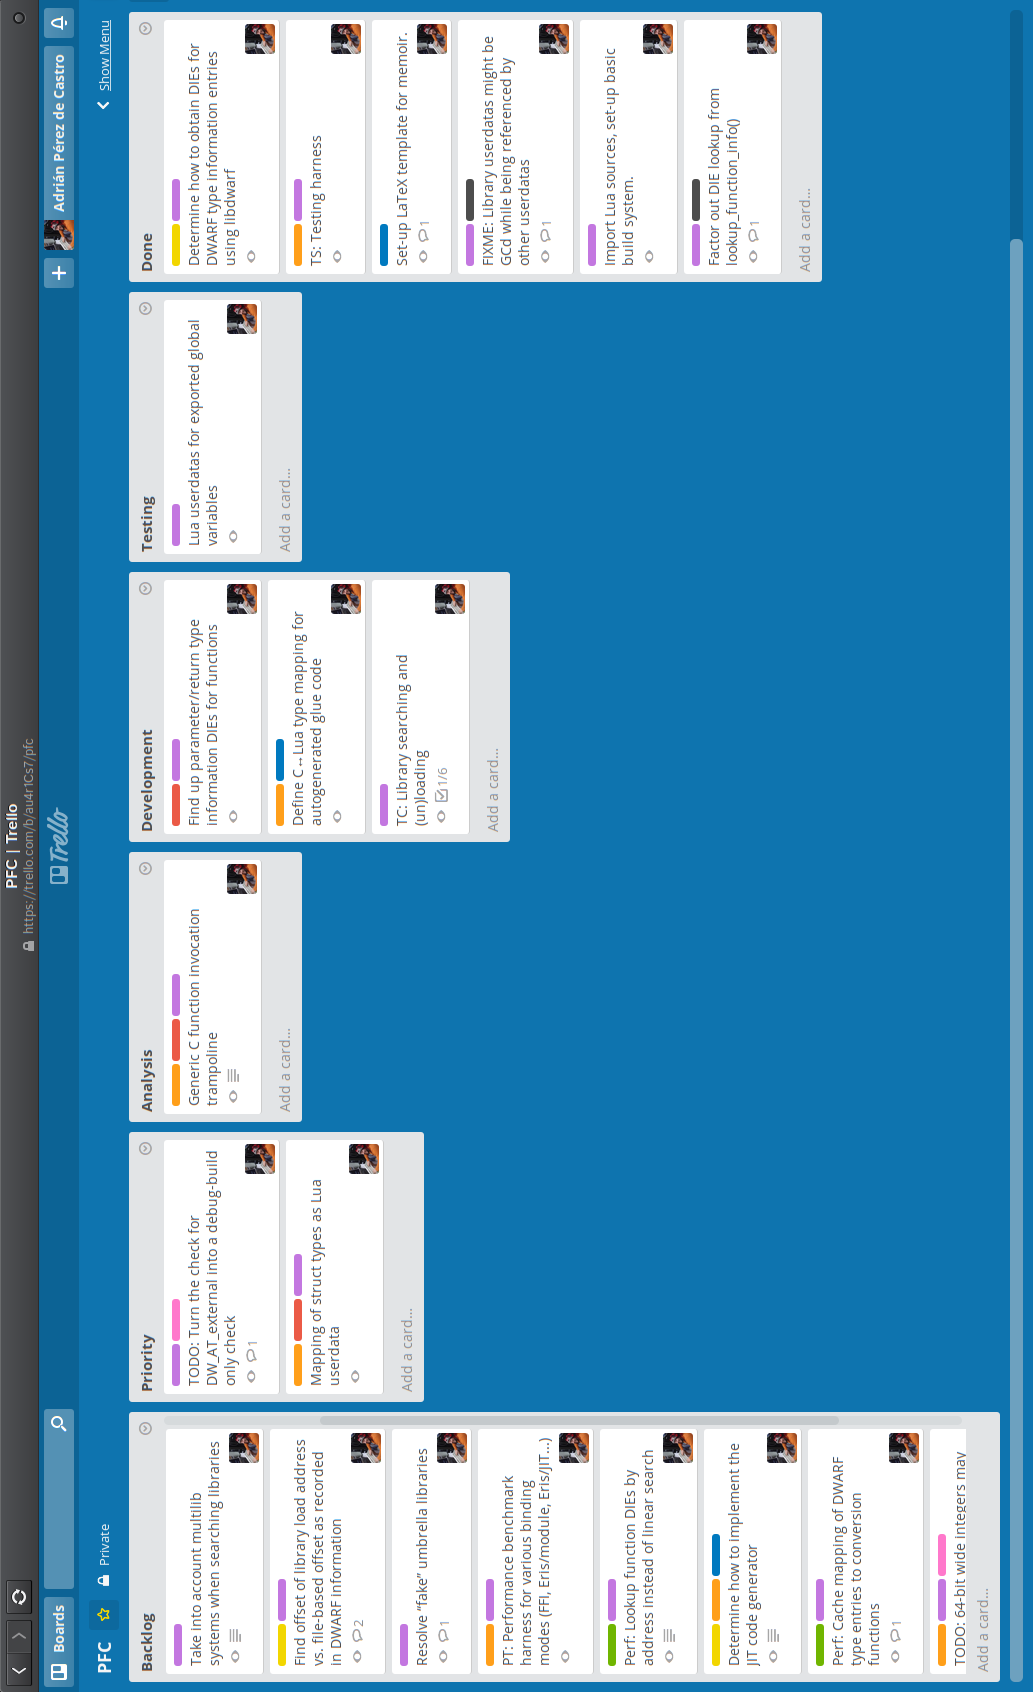
\includegraphics[width=0.8\textwidth]{img/trello-board.png}
	\caption{Kanban board, showing some tasks of this very project}
	\label{fig:kanban-board}
\end{figure}

The Kanban method was invented by \gls{Toyota} to keep the status of
production lines. This methodology keeps a board (physical, in the original
incarnation of the method; nowadays there are even web-based applications like
the one shown in \autoref{fig:kanban-board}) where each element is a task, and
elements are distributed in columns depending on their status. For example,
applied to software development, the columns could be “Pending”, “In
Progress”, “Testing”, and “Finished”. All the tasks are always visible in the
board, so this allows to know the overall status of a project intuitively by
glancing at the board.


\beforeintro

% vim: ft=tex spell spelllang=en ts=2 sw=2

\cleardoublepage
\setchaptertoc
\chapter{Contextualization}

Computing would not be understood without the accompanying tools which enable
IT professionals to actually \emph{do something} with computers: from simple
switches and lights in the early times, to the sophisticated programming
languages and tools of the present times, all of them enable humans to
\emph{instruct machines to do things}. This chapter introduces the tools and
concepts involved in the realization of this project.
\afterintro

%% TODO

\section{Dynamic Programming Languages}

Dynamic languages~\cite{tratt-dynamic-langs} are a family of high-level
programming languages which, at runtime, execute programming behaviors that
other programming languages perform during compilation. Runtime behaviors
could include extension of the program, by adding new code, by extending
objects and definitions, or by modifying the type system. Support for these
operations is provided directly by the language. Most dynamic languages are
also dynamically typed, and are frequently called “scripting languages”.

Popular contemporary scripting languages include Perl, Python, PHP, the
ubiquitous JavaScript, and of course Lua (described in
\autoref{sec:lua-programming-lang}). Many of their features were first
implemented as native features of the Lisp programming language, which itself
is dynamic.

Dynamic programming languages have grown in popularity in the last decades.
Programmers like them for their expressiveness, which allows for higher
productivity, and the ever increasing computing power of computers makes it
feasible to use them for performance-critical tasks traditionally left for
statically compiled languages. The development of novel compilation techniques
aimed at this family of languages, and the relentless improvement of their
virtual machines (see \autoref{sec:virtual-machines}), has contributed as well
to increase widespread adoption.

\subsection{Virtual Machines as Runtime Environments}
  \label{sec:virtual-machines}

A \gls{VM} is an \gls{emulation} of a particular computer system based on its
architecture. \emph{System virtual machines} provide a complete substitute for
the real machine, and targeted towards the execution of complete operating
systems and software stacks. On the other hand, \emph{process virtual
machines} execute a single computer program by providing an execution
environment suitable for a particular programming language, which can be
platform-independent.

Process \gls{VM}s provide a so called \emph{runtime environment}. They run as
a normal application inside the host operating system. This approach has
several advantages:

\begin{itemize}
	\item Provides a platform-independent programming environment,
		abstracting away details of the underlying hardware or operating system,
		potentially allowing a program to execute in the same way on any platform.
	\item The level of abstraction provided by the \gls{VM} is higher than that
		of a low-level \gls{ISA}, which allows it to provide services rarely
		available in real machines (e.g. automatic memory management).
	\item There is an additional level of isolation between the operating system
		and the execution environment. This allows discretionary control over the
		executed code, which is confined to the bounds allowed by the \gls{VM}.
\end{itemize}

The main downside of virtual machines is the lower performance compared to the
execution of native code. Performance levels comparable to compiled languages
can be obtained using a combination of \gls{JIT} compilation (see
\autoref{sec:jit-compilers}), and compiler-based optimization techniques
specifically designed for them.

In some regards, the additional level of isolation provided by a \gls{VM}
could be a nuisance due to the fact that it could prevent programs from
accessing resources (either hardware-based, or provided by the host system)
needed for its operation. For this reason, many virtual machines provide
a \gls{FFI}: a mechanism to call-out native code and re-gain access to the
whole system, while still being under the control and supervision of the
\gls{VM}.


\subsection{JIT Compilers}
	\label{sec:jit-compilers}

% TikZ styles for box diagrams
\tikzstyle{bdBox} = [
	rectangle, drop shadow, draw=black, thick, fill=white,
	text centered, minimum height=2em, minimum width=3em,
]
\tikzstyle{bdProcBox} = [
	rounded corners, fill=blue!10, text centered
]
\tikzstyle{bdProcLine} = [
	draw, thick, color=blue!20
]
\tikzstyle{bdCircle} = [
	circle, fill=blue!20, draw=black,
]
\tikzstyle{bdLine} = [draw, thick]
\tikzstyle{bdArrow} = [bdLine, >=triangle 45, ->]

\begin{figure}[ht]
	\centering
	\begin{tikzpicture}[node distance=1.4cm]
		\small
		\node[bdBox] (srcbox) [start chain=going right, on chain] {Source code};
		\node[bdCircle] (aot) [on chain] { };
		\node[bdProcBox] (aotlabel) [below of=aot] { \emph{Basic JIT compilation} };
		\node[bdBox] (bytecode) [on chain] {Bytecode};
		\node[bdCircle] (jit) [on chain] { };
		\node[bdProcBox] (jitlabel) [below of=jit] { \emph{Optimizing JIT compilation} };
		\node[bdBox] (bincode) [on chain] {Machine code};

		\node (profileinfo) [above of=bytecode, xshift=1cm] {Runtime statistics};

		\path[bdLine] (srcbox.east) -- (aot.west);
		\path[bdArrow] (aot.east) -- (bytecode.west);
		\path[bdLine] (bytecode.east) -- (jit.west);
		\path[bdArrow] (jit.east) -- (bincode.west);
		\path[bdLine] (profileinfo) -- (jit);

		\path[bdProcLine] (aot.south) -- (aotlabel.north);
		\path[bdProcLine] (jit.south) -- (jitlabel.north);
	\end{tikzpicture} \caption{Two-tier JIT compilation}
	\label{fig:two-tier-jit} \end{figure}

\acrlong{JIT} compilation is a term which refers to any technique that
performs compilation of program code during the execution of the program —at
runtime—, instead of doing it before execution. This is also known as
\emph{dynamic translation}. Typically a VM which uses JIT compilation contains
two compilers (\autoref{fig:two-tier-jit}):

\begin{enumerate}

		\item The first compiler —known as \emph{tier 1}— performs a translation
		of the input source code into an intermediate binary representation known
		as \emph{bytecode}, which is faster to execute than interpreting the
		source code in its original form. In order to start executing the
		program as quickly as possible, this first compiler performs only basic
		optimizations—if any. Additionally, the compiler adds instrumentation code
		in the generated bytecode, which gathers statistics about program execution.
		
		\item The second compiler —known as \emph{tier 2}— generates either
		bytecode which is better optimized, or machine code, at the cost of
		slower compilation speed, compared to the tier 1 compiler. The
		statistics gathered by the instrumentation code inserted by the tier
		1 compiler are used to determine which parts of the program code are used
		more often, and only those are recompiled. Depending on the
		implementation, compilation is done per source file, per function, or even
		for arbitrary code fragments. The bytecode produced by the tier 1 compiler
		can be used as input to avoid having to re-parse the program source code
		in its textual form.

\end{enumerate}
		
Some VMs do not provide a bytecode interpreter, and must always generate
machine code. In this scenario, the tier 1 compiler also generates machine
code, but unoptimized to avoid having long delays during the startup process
of the VM when the tier 1 compiler is used.

Code generated by JIT compilers offers better performance than interpreters,
and in some cases it can perform better than statically compiled code because
a JIT compiler can use optimizations which are only feasible at runtime:

\begin{itemize}

	\item Generated code can be optimized for the exact processor and operating
	system where the application runs. This can be done with traditional
	compilers, but it requires compiling the code once for each combination of
	target processor and operating system.

	\item The VM can collect statistics about how the program is running, and
	rearrange and recompile the code according to them.

	\item The compiler can make optimistic assumptions about the program,
	generate machine code that works optimally in most of the situations, plus
	additional checks to know whether the assumptions hold, falling back to
	using the original implementation (or a different re-compilation) otherwise.
	For example, this strategy is used to inline method calls assuming that
	\gls{dynamic-dispatch} will not be needed, and performing the dynamic
	dispatch when the types of the involved objects to not match the ones assumed.

	\item Code can be rearranged after observing how it uses the cache memory to
	make a better usage of it.

\end{itemize}

The introduction of JIT compilation in VMs has allowed existing dynamic
languages to achieve levels of performance comparable to those of languages
compiled to machine code~\cite{lj-perf1}. The JavaScript programming language
is a paradigmatic example: it has existed since 1995, yet it has gained much
more widespread usage after the introduction in 2008 of JavaScript engines
capable of JIT compilation (Mozilla's TraceMonkey was the first, with Google's
V8 and WebKit's JavaScriptCode following right after~\cite{js-raceforspeed}),
making it feasible to use JavaScript as a general purpose language outside of
web browsers.


\subsection{The Lua programming language}
	\label{sec:lua-programming-lang}

The Lua language is a “powerful, fast, lightweight, embeddable scripting
language” \cite{lua-about}. It was initially created as a data description
language at \gls{PUC-Rio}, to be used for in-house software development, and
has since evolved into a general purpose programming language. It has been
used in proffessional applications (e.g. Adobe Lightroom) and it has seen
widespread usage in the video games industry (e.g. World Of Warcraft).

\begin{listing}[htH]
  \begin{luacode}
    fib = { 1, 1 }
    setmetatable(fib, {
      __index = function (values, n)
        -- Calculate and memoize the Fibonacci(n)
        values[n] = values[n - 1] + values[n - 2]
        return values[n]
      end
    })
    print(fib[10])  --> 55
  \end{luacode}
  \caption{\Gls{memoization} and \gls{dynamic-programming} using a Lua metatable}
	\label{lst:lua-example-memoize}
\end{listing}

Lua's main programming paradigm is imperative, but the language supports
functions as \glspl{first-class-value} and \glspl{closure}, making it possible
to easily write programs in a functional programming style. Like in
\gls{pascal}, English words (\Mlua|function|, \Mlua|then|, \Mlua|end|) are
used as delimiters for language constructs. Another defining characteristic of
the language is that, by design, it only provides one compound data structure,
the \emph{table}, which is the basis for all user--defined types. Tables can
be used as arrays (\autoref{lst:lua-example-memoize}), structures, and
objects (\autoref{lst:lua-example-tables}).

\begin{listing}[htH]
  \begin{luacode}
    -- Create a table, with one key, "age" and 7 as value
    animal = { age = 7 }

    -- Associate a string value to the "kind" table key
    animal["kind"] = "cat"

    -- Keys which are valid identifiers can be accessed with "."
    animal.name = "Doraemon"

    -- The dot "." syntax workds for adding functions to tables
    function animal.describe(self)
      print(self.name .. " is a " .. tostring(self.age) ..
            "-year old " .. self.kind)
    end

    -- This is equivalent to: animal.describe(animal)
    animal:describe()  --> Doraemon is a 7-year old cat

    -- Adding a function with colon ":" adds an implicit "self"
    function animal:furryness()
      return self.kind == "cat" and "high" or "unknown"
    end

    animal:furryness()  --> high
  \end{luacode}
	\caption{Lua tables being used as objects}
  \label{lst:lua-example-tables}
\end{listing}


A unique and powerful feature of Lua is its support for \emph{metatables}:
values may have an associated table (the so-called \emph{metatable}) which
allows to extend the semantics of language constructs, allowing to define how
tables behave when arithmetic and relational operators are applied to tables,
or how table fields are accessed. \autoref{lst:lua-example-memoize}
demostrates how customizing table access can be used to define a
seemingly--infinite array which contains the $n^{th}$ \gls{fibonacci-number}
at index $n$. A common use for metatables is enabling support for
object--oriented programming, using them to define object inheritance chains
(\autoref{lst:lua-example-meta-oo}) --- as Lua itself does not have the
notion of classes, prototypes are used instead, as in the Self or JavaScript
languages.

\begin{listing}[htH]
  \begin{luacode}
    -- Base object describing an unnamed living creature
    animal = {
      name = "Unnamed",
      kind = "living creature",
      describe = function (self)
        print(self.name .. " is a " .. self.kind)
      end,
    }

    -- When indexing the table passed as first argument, fields will
    -- be looked up from the "animal" table associated to the "__index"
    -- key of the metatable. The function returns the first argument.
    cat = setmetatable({ kind = "cat", name = "Doraemon" },
                       { __index = animal })
    dog = setmetatable({ kind = "dog", name = "Snowy", },
                       { __index = animal })

    -- The :describe() method is searched in "animal"
    cat:describe()  --> Doraemon is a cat
    dog:describe()  --> Snowy is a dog

    -- Chained key lookup can be used to make the values from the
    -- base object the default ones
    tom = setmetatable({ name = "Tom" }, { __index = animal  })
    tom:describe()  --> Tom is a living creature
  \end{luacode}
  \caption{Lua metatables used for object inheritance}
  \label{lst:lua-example-meta-oo}
\end{listing}

Lua, starting in version 5.0~\cite{lua50-impl}, uses a register-based virtual
machine. This allows for improved performance by avoiding excessive copying of
values on stack \emph{pop} and \emph{push} operations. Traditionally, most
virtual machines intended for execution of languages are stack based,
including heavyweight, enterprise-proven systems like the Java™ JVM, and
Microsoft's .NET environment.


\section{Binding Native Code to Lua}

\subsection{Lua C API}
	\label{sec:lua-c-api}

The Lua \gls{VM} exposes a C \gls{API} which, among other things, allows to
register C functions to be called by Lua code. These communicate with the VM
using a well-defined protocol (see \autoref{lst:lua-c-api-example}
for an example).

\begin{listing}[htH]
	\begin{ccode}
  int sum_and_average (lua_State *L) {
    lua_Number result = 0.0;
    int nargs = lua_gettop (L); /* number or arguments */
    for (int i = 1; i <= n; i++) {
      if (!lua_isnumber (L, i)) {
        lua_pushliteral (L, "argument is not a number");
        lua_error (L);
      }
      result += lua_tonumber (L, i);
    }
    lua_pushnumber (L, result);        /* first result */
    lua_pushnumber (L, result / n);   /* second result */
    return 2;                     /* number of results */
  }
	\end{ccode}
	\caption{C function callable from Lua}
	\label{lst:lua-c-api-example}
\end{listing}

Despite Lua providing a register-based VM, the C API uses a \emph{virtual
stack} to exchange values with C code. When a C function is called, it gets
a new stack, initially containing the arguments passed to the function, and
it must adhere to the following protocol:

\begin{itemize}
	\item C functions must be declared as returning an \Mc|int|, and accept
		a single \Mc|lua_State*| parameter. This is, their function pointer
		type is compatible with \Mc|lua_CFunction|, which Lua defines as:
		\begin{ccode}
			typedef int (*lua_Cfunction) (lua_State*);
		\end{ccode}

	\item The C function receives arguments from Lua in its call stack in
		direct order (the first argument is pushed first by the VM). The size of
		the stack —at this point the number of arguments— can be queried using
		\Mc|lua_gettop()|, and values can be obtained using the \verb|lua_to*()|
		functions.

	\item To return values back to Lua, the C function pushes them onto the
		stack in direct order (the first result is pushed first) using the
		\verb|lua_push*()| functions.

	\item The C function passes control to the VM returning the number of
		results available at the top of the stack. Any values left in the
		stack below the results are discarded.

\end{itemize}

Values of data managed by native code can be handled by the Lua VM as
\emph{userdata}. Even though userdata values are opaque to Lua, setting their
metatable allows the programmer to define their behavior using the same
language (e.g. C, C++) from which the VM is embedded. This is crucial for
avoiding data corruption, as it can only be manipulated by native code in
the way the programmer intended. See
\autoref{sec:userdata-lua-custom-allocator} for additional discussion
on this topic.

The C API provided by Lua is comprehensive, but using it tends to produce
verbose programs, with varying amounts of repeated code. Lua itself
acknowledges this issue by officially including an \emph{auxiliar library}
as part of the package, which provides a collection of utility functions
implemented using the base API. Third-party wrappers over the official API
exist, which can either provide a more convenient interface to Lua (like
LuaAutoC\footnote{\url{https://github.com/orangeduck/LuaAutoC}}, and
\verb|luapi|\footnote{\url{http://lua-users.org/files/wiki_insecure/users/luapi/luapi5-1.txt}}),
or allow languages other than C to use Lua (more than
20 at the time of writing, including support for many popular languages like
C++, Objective-C, Go, Java, or Fortran).


\subsection{Binding Generators}
	\label{sec:binding-generators}

Binding generators are tools that can be used to create a binding to a library
in an automated way. Often they fall into the category of \glspl{transpiler}:
they take as input the source code of the code to generate a binding for,
and generate a new set of source files which contain the code of the binding.
This set of source files are themselves compiled into a loadable module for
the target programming language or virtual machine, making it a
\emph{build-time} solution.

More than often, binding generators do \emph{not} include a full parser for
the programming language of origin, and they require to be fed a simplified
version of the code being wrapped. This can be a nuisance for code bases which
use complex language constructs unsupported by the binding generator.

A popular, general-purpose binding generator is
SWIG\footnote{\url{http://swig.org}} (Simple Wrapper and Interface Generator),
which supports creating bindings for multiple programming languages, with Lua
being just one more of the supported targets. SWIG uses its own C/C++ parser,
which, while being complete~\cite{swig3doc}, still fails on certain inputs.

There are also Lua-specific binding generators, of which the
\gls{lua-users-wiki} provides a comprehensive
list~\cite{lusers-BindingCodeToLua}. The oldest is
ToLua\footnote{\url{http://www.tecgraf.puc-rio.br/~celes/tolua/}}, maintained
by staff from \gls{PUC-Rio} like Lua itself. Being Lua the only target
language, bindings generated by ToLua —and derivatives like ToLua++— are more
idiomatic that those generated by e.g. SWIG. As a downside, ToLua's parser is
quite limited, and only recognizes a subset of C and C++, to the point that it
is advised to provide a \emph{cleaned header file} containing only
declarations of data types, functions, and C++ classes recognizable by its
parser.


\subsection{Foreign Function Interfaces}
	\label{sec:ffis}

In its most generic meaning, a \gls{FFI} is any mechanism which allows
a program written in a programming language to call code or use services
written in another. In the Lua community, a FFI refers specifically to such
a mechanism which works at run time. That is, it \emph{does not} require using
the Lua C API (\autoref{sec:lua-c-api}), it is not a binding generator used at
build time (\autoref{sec:binding-generators}), nor is it a wrapper over the
Lua C API.

FFIs can be separated in two categories, depending on how they obtain the type
information (functions names, arguments, return values; and the data types of
all the values involved):

\begin{itemize}

	\item FFIs which require the programmer to supply type information.

	\item FFIs which obtain type information in an automated fashion.

\end{itemize}

The canonical example of a FFI which requires the programmer to enter type
information is the \gls{LuaJIT} FFI
module\footnote{\url{http://luajit.org/ext_ffi.html}}. Its functionality is
available as a regular Lua module which includes a number of support
functions, including the ability to parse C-style declarations to obtain type
information. Under the hood, the module generates the machine code for wrapper
functions —of type \Mc|lua_CFunction| (c.f. \autoref{sec:lua-c-api})— using
the LuaJIT code generator, which are directly callable (example in
\autoref{lst:luajit-ffi-example}). A standalone
\verb|luaffi|\footnote{\url{https://github.com/jmckaskill/luaffi}} module for
the standard Lua \gls{VM} exists, which has the same interface as the LuaJIT
FFI module, and even reuses its code generator.

\begin{listing}[H]
	\begin{luacode}
  local ffi = require("ffi")
  ffi.cdef("int printf(const char *fmt, ...);")
  ffi.C.printf("Hello %s!\n", "world")
	\end{luacode}
	\caption{Using a C function with the LuaJIT FFI}
	\label{lst:luajit-ffi-example}
\end{listing}

Where the LuaJIT FFI requires the programmer to enter C-style declarations of
functions, LGI\footnote{\url{https://github.com/pavouk/lgi/}} uses the type
information supplied by GObject Introspection~\cite{gobject-introspection},
which provides access to most of the libraries included as part of the
GNOME\footnote{\url{http://gnome.org}} desktop environment. The type
information supplied by GObject Introspection is extracted from the source
code of the GNOME destop components at compile-time, and stored on disk in its
own file format. The included \verb|libgirepository| library is then used by
LGI to allow the enumeration of the available modules and their contents, as
well as the transparent invocation of functions from Lua. The metadata
recorded by GObject Introspection when scanning source code includes
additional information in specially formatted comments, which allows LGI to
create idiomatic object oriented interfaces (c.f. \autoref{lst:lua-lgi-example}).

\begin{listing}[H]
	\begin{luacode}
	local lgi = require("lgi")
	local Gtk = lgi.Gtk

	local w = Gtk.Window {
		title = "LGI Example",
		child = Gtk.Button { label = "Close",
                         on_clicked = Gtk.main_quit },
	}
	w:show_all()
	Gtk.main()
	\end{luacode}
	\caption{Using the GTK+ user interface toolkit via LGI and GObject
	Introspection}
	\label{lst:lua-lgi-example}
\end{listing}

\section{Executable Formats}

\subsection{ELF}
  \label{sec:elf}

The \acrlong{ELF} (ELF, formerly called \emph{Extensible Linking
Format}) is a common standard file format for executable programs, object
code, shared libraries, and even core dumps. Since its publication as part of
the System V Release 4 (SVR4) Application Binary Interface (ABI) specification
\cite[c.~4]{elfspec-sysv}
it has been adopted by many Unix-like (Solaris, most of the BSD variants,
GNU/Linux), and non-Unix operating systems (most notably, OpenVMS, BeOS, and
its successor Haiku).

\noindent An ELF file contains three mandatory parts
(\autoref{fig:elf-structure}):

\begin{itemize}

	\item The ELF header, which contains general information about the file
	(architecture, endianness, ABI, etc.), the offsets of the \emph{program
	header table}, and the \emph{section header table}; and their sizes.

	\item The \emph{program header table}, which describes zero or more
	\emph{segments}. Though it is not required, it is typically located right
	after the ELF header.

	\item The \emph{section header table}, which describes zero or more
	\emph{sections}.

\end{itemize}

\begin{figure}
	\centering
	\begin{tikzpicture}[node distance=1.5mm, bend angle=0]
		\small
		\node[bdBox] (elfheader) [minimum width=10em, start chain=going below, on chain] {ELF header};
		\node[bdBox] (prgheader) [minimum width=10em, on chain] {Program header};
		\node[bdBox] (sect-text) [minimum width=10em, on chain] {\verb|.text|};
		\node[bdBox] (sect-rodata) [minimum width=10em, on chain] {\verb|.rodata|};
		\node (ellipsis) [minimum width=10em, on chain, yshift=-1em] {...};
		\node[bdBox] (sect-data) [minimum width=10em, on chain, yshift=-1em] {\verb|.data|};
		\node[bdBox] (secthdrtable) [minimum width=10em, on chain] {Section header table};

		\draw[decorate, decoration={brace}] let \p1=(sect-text.north),
			\p2=(sect-rodata.south) in ($(2.2, \y1)$) -- ($(2.2, \y2)$)
			node[midway] (g1) {};

		\draw[decorate, decoration={brace}] let \p1=(ellipsis.north),
			\p2=(sect-data.south) in ($(2.2, \y1)$) -- ($(2.2, \y2)$)
			node[midway] (g2) {};

		\draw[->, bend right, >=latex, bend right, thick]
			(elfheader.east) to [out=90,in=90] (g1.east);
		\draw[->, bend right, >=latex, bend right, thick]
			(elfheader.east) to [out=90,in=90] (g2.east);

		\draw[->, bend left, >=latex, bend right, thick]
			(secthdrtable.west) to [out=90,in=90] (sect-text.west);
		\draw[->, bend left, >=latex, bend right, thick]
			(secthdrtable.west) to [out=90,in=90] (sect-rodata.west);
		\draw[->, bend left, >=latex, bend right, thick]
			(secthdrtable.west) to [out=90,in=90] (sect-data.west);
	\end{tikzpicture}
	\caption{Structure of an ELF object file}
	\label{fig:elf-structure}
\end{figure}

Consequently, with the aforementioned parts of an ELF file, the actual data is
categorized in \emph{segments}, and \emph{sections}. Segments contain
information used at runtime for the execution of the code, and sections
contain data about the code itself. Section names and contents are arbitrary,
and they are used to store information used \emph{offline} (i.e. not at
runtime) needed for relocating and linking the program code contained in the
ELF file.

Entries for both program and section header tables contain the sizes of the
segments and sections they describe, and their offsets inside the ELF file. It
is allowed by the specification to define more than one segment and section
entries which refer to the same portion of the file, and also that there are
portions of the file which do not belong to any segment or section.


\subsection{DWARF}

% The DWARF debugging information format has been designed along with
% ELF\footnote{And that is why both have names related to the medieval fantasy
% canon.}, although it is possible to store DWARF-encoded data in other object
% file formats. The DWARF specification~\cite{dwarfspecv4} defines how to encode
% all kinds of information potentially useful for a debugger, and how it must be
% laid out in different object code file formats.
%
% Each piece of information encoded in DWARF is stored in \gls{DIE}. Each DIE is
% a data records with a \emph{tag} which determines the type of information
% represented, and a payload which varies depending on the value of the tag.
% When a DIE is used to describe a data type, it is often referred to as
% a \gls{TUE}.
%
% DIEs are the  In the case of ELF files (\autoref{sec:elf}), the DWARF
% information is laid out inside the ELF file in a number of sections
%
% \begin{itemize}
%
% 	\item The \verb|.debug_info| section contains 
%	
% 	and \verb|.debug_types| sections contain a number of data records which
% 	describe the different entities present in the program, and their data
% 	types. Each one of those records is called a \gls{DIE}.
%
% \end{itemize}

The \gls{DWARF} format was first developed by the Bell Labs for the
\verb|sdb| debugger of System V Unix. Nowadays the formal specification
is available under the GNU \gls{FDL}, and its new versions have been
discussed using public channels of communication, following a
community-oriented process. Downloadable copies of all the version of
the specification are available at {\small\url{http://dwarfstd.org}}.

Debugging information is not strictly needed at runtime for the execution of
the program: it is considered ancillary, and therefore is stored in sections.
As per the specification, the DWARF debugging information must be stored in
the ELF objects in sections with the \verb|.debug_| prefix. Each one of those
sections stores a particular kind of information, as seen on
\autoref{tab:elf-dwarf-sections}.

\begin{table}
  \centering\small
  \begin{tabular}{lp{0.65\textwidth}}
    \toprule
    Section & Contents \\
    \midrule
    \verb|.debug_types| & Stores DIEs for types. \\
    \verb|.debug_info| & Stores DIEs for executable program code (functions, mostly) \\
    \verb|.debug_line| & Maps of object code positions to source code line numbers \\
    \verb|.debug_pubnames| & Public function names and entry offsets in \verb|.debug_info| \\
    \verb|.debug_pubtypes| & Public type names and entry offsets in \verb|.debug_types| \\
    \verb|.debug_str| & String data (e.g. type, variable and function names) \\
    \bottomrule
  \end{tabular}
  \caption{Main ELF sections used to store DWARF debugging information}
  \label{tab:elf-dwarf-sections}
\end{table}


In \gls{DWARF}, all the data provided by debugging information is stored in
a hierarchical tree-like structure, and each node of the tree is called
a \gls{DIE}. Each DIE consists of an identifying tag, and a series of
attributes. The tag specifies the class to which an entry belongs, and the
attributes define the characteristics of the entry. An entry, or a group of
entries together, provide a description of an entity in the corresponding
source code. The entries are contained in the \verb|.debug_info| and
\verb|.debug_types| sections of ELF object files.

%%%
%%% TikZ styles for DIE diagrams
%%%
\pgfdeclarelayer{background}
\pgfdeclarelayer{foreground}
\pgfsetlayers{background,main,foreground}

\tikzstyle{datablob} = [
  rectangle, rounded corners, drop shadow, draw=black, thick,
  text centered, minimum height=2em, minimum width=3em, fill=blue!20,
]
\tikzstyle{die}      = [start chain=going below, node distance=1mm]
\tikzstyle{dielabel} = [on chain]
\tikzstyle{dieitems} = [
  rectangle split, rectangle split parts=#1, rectangle split part align=left,
  thick, draw, fill=blue!10, on chain,
]
\tikzstyle{enumitems} = [
  rectangle split, rectangle split parts=#1, rectangle split part align=left,
  thick, rounded corners,
  color=black!50, fill=black!5, draw=black!50,
  minimum height=3em,
]
\tikzstyle{valuefrom} = [draw=black!50, thick, dashed]
\tikzstyle{arrow} = [draw, thick, >=triangle 45, ->]
\tikzstyle{datain} = [
  draw=black!80, thick, fill=blue!10, rectangle,
  text centered, minimum height=1.3em, text width=10em,
]
%%%
%%% End TikZ styles for DIE diagrams
%%%

\begin{figure}
  \centering
  \begin{tikzpicture}[die]
    \node[dielabel] (taglabel) {Tag};
    \node[dieitems=1] (tag) {\verb|DW_TAG_subprogram|};

    \node[dielabel] (attrlabel) {Attributes};
    \node[dieitems=3] (attributes) {
        \verb|DW_AT_type|
      \nodepart{two}
        \verb|DW_AT_sibling|
      \nodepart{three}
        \verb|DW_AT_…|
    };

    \node[datablob] (refdie2) [right=4cm of attributes] { };
    \node[datablob] (refdie1) [above=1mm of refdie2] { };
    \node  (refdieellipsis)   [below=1mm of refdie2] { ... };
    \node[datablob] (refdieN) [below=1mm of refdieellipsis] { };

    \node (refdieslabel) [above=3mm of refdie1] {DIEs referenced by offset};

    \path[arrow] (attributes.text east) -- (refdie1.west);
    \path[arrow] (attributes.two east) -- (refdie2.west);
    \path[arrow] (attributes.three east) -- (refdieN.west);

    \begin{pgfonlayer}{background}
      \node[datablob] (die) [fit=(taglabel) (attributes) (tag)] { };
      \node[fill=yellow!20, rectangle, rounded corners] (refdiesbg)
        [fit=(refdieslabel) (refdieN)] { };
    \end{pgfonlayer}

    \node (dielabel) [below=3mm of die] {DIE};
  \end{tikzpicture}

  \caption{DIE attribute references.}
  \label{fig:die-attr-references}
\end{figure}

DIE attributes can contain references to other DIEs, as shown in
\autoref{fig:die-attr-references}, making it possible to create arbitrary
links between nodes of the tree. Those explicit links are used extensively to
group related entries together (for example entries with tag
\verb|DW_TAG_formal_parameter|, which describe the parameters of a function,
are chained using \verb|DW_AT_sibling| attributes), and to perform
\gls{data-deduplication} of the debug information (for example, instead of
making a new entry for the \mintinline{c}{int} type, only one is created and
then referenced from other entries).


\label{sec:debuginfo-structure}

We now provide a simplified overview of the tree structure formed by the debug
information entries of a program, in a level of detail which is enough for the
goals of this project. For complete, detailed information, we refer to the
DWARFv4 Specification~\cite{dwarfspecv4}.


\subsubsection{Types}

A type is represented as a DIE with one of the following tags:

\begin{itemize}
  \item \verb|DW_TAG_base_type|
  \item \verb|DW_TAG_pointer_type|
  \item \verb|DW_TAG_typedef|
  \item \verb|DW_TAG_const_type|
  \item \verb|DW_TAG_array_type|
  \item \verb|DW_TAG_structure_type|
  \item \verb|DW_TAG_union_type|
  \item \verb|DW_TAG_enumeration_type|
\end{itemize}


\minisec{Base Types}

\begin{figure}
  \centering
  \begin{tikzpicture}[die]
    \node[dielabel] (taglabel) {Tag};
    \node[dieitems=1] (tag) { \verb|DW_TAG_base_type| };
    \node[dielabel] (attrlabel) {Attributes};
    \node[dieitems=2] (attributes) {
        \verb|DW_AT_byte_size|
      \nodepart{second}
        \verb|DW_AT_encoding|
    };

    \node[enumitems=1] (sizevalues) [right=4cm of tag] {\emph{size}};
    \node[enumitems=4] (encodingvalues) [below=1cm of sizevalues] {
        \verb|DW_ATE_signed|
      \nodepart{second}
        \verb|DW_ATE_unsigned|
      \nodepart{third}
        \verb|DW_ATE_float|
      \nodepart{fourth}
        \verb|DW_ATE_boolean|
    };

    \path[valuefrom] (attributes.text east) -- (sizevalues.west);
    \path[valuefrom] (attributes.second east) -- (encodingvalues.west);

    \begin{pgfonlayer}{background}
      \node[datablob] [fit=(taglabel) (attributes) (tag)] {};
    \end{pgfonlayer}
  \end{tikzpicture}
  \caption{DIE describing a base type.}
  \label{fig:die-base-type}
\end{figure}


Base types(\autoref{fig:die-base-type}) are represented by DIEs with
a \verb|DW_TAG_base_type| tag. This covers all the C/C++ numeric types: signed
and unsigned integers, floating point types (\mintinline{c}{float},
\mintinline{c}{double}), the \mintinline{c}{char} type, and the new
integer-based types of C99 (\mintinline{c}{_Bool}, \mintinline{c}{int32_t},
etc.)

The size of the values is given using a \verb|DW_AT_byte_size| attribute,
in bytes. Sizes are the same reported by the C \mintinline{c}{sizeof}
operator. A \verb|DW_AT_encoding| attribute specifies how the values are
used in the program. For example, \verb|DW_ATE_boolean|
corresponds with the \Mc|bool| type (or \Mc|_Bool|) in the
source program. \autoref{tab:dwarf-base-types-mapping} summarizes how C
types are represented by a base type DIE for the x86\_64 architecture
(sizes may vary in other architectures).

\begin{table}[ht]
	\begin{center}
		\begin{tabular}{lcl}
			\toprule
			C Type & \verb|DW_AT_byte_size| & \verb|DW_AT_encoding| \\
			\midrule
			\mintinline{c}{bool}               & 1 & \verb|DW_ATE_boolean| \\
			\mintinline{c}{char}               & 1 & \verb|DW_ATE_signed_char| \\
			\mintinline{c}{unsigned char}      & 1 & \verb|DW_ATE_unsigned_char| \\
			\mintinline{c}{short int}          & 2 & \verb|DW_ATE_signed| \\
			\mintinline{c}{unsigned short int} & 2 & \verb|DW_ATE_unsigned1| \\
			\mintinline{c}{int}                & 4 & \verb|DW_ATE_signed| \\
			\mintinline{c}{unsigned int}       & 4 & \verb|DW_ATE_unsigned| \\
			\mintinline{c}{long int}           & 8 & \verb|DW_ATE_signed| \\
			\mintinline{c}{unsigned long int}  & 8 & \verb|DW_ATE_unsigned| \\
			\mintinline{c}{float}              & 4 & \verb|DW_ATE_float| \\
			\mintinline{c}{double}             & 8 & \verb|DW_ATE_float| \\
			\mintinline{c}{long double}        & 16& \verb|DW_ATE_float| \\
			\bottomrule
		\end{tabular}
	\end{center}
	\caption{DWARF representation of C base types for the x86\_64 architecture}
	\label{tab:dwarf-base-types-mapping}
\end{table}

The rest of C/C++ base types are defined as aliases of these
using \mintinline{c}{typedef}.


\minisec{Pointer Types}

\begin{figure}
  \centering
  \begin{tikzpicture}[die]
    \node[dielabel] (taglabel) {Tag};
    \node[dieitems=1] (tag) {\verb|DW_TAG_pointer|};
    \node[dielabel] (attrlabel) {Attributes};
    \node[dieitems=1] (attributes) {\verb|DW_AT_type|};

    \node[dielabel] (rtaglabel) [right=3cm of tag, yshift=-3.5mm] {Tag};
    \node[dieitems=1] (rtag) {\verb|DW_TAG_pointer|};
    \node[dielabel] (rattrlabel) {Attributes};
    \node[dieitems=1] (rattributes) {\verb|DW_AT_type|};

    \node[datablob] (basedie) [right=2cm of rattributes] {Type DIE};

    \path[arrow] (rattributes.text east) -- (basedie);

    \begin{pgfonlayer}{background}
      \node[datablob] (die) [fit=(taglabel) (attributes) (tag)] {};
      \node[datablob] (rdie) [fit=(rtaglabel) (rattributes) (rtag)] {};
    \end{pgfonlayer}

    \path[arrow] (attributes.text east) -- (rdie.west);
  \end{tikzpicture}
  \caption{DIEs describing a Pointer-to-pointer-to type.}
  \label{fig:die-pointer-type}
\end{figure}

Pointer types (\autoref{fig:die-pointer-type}) are represented by DIEs with
a \verb|DW_TAG_pointer_type| tag, and a lone \verb|DW_AT_type| attribute
points to the DIE of the pointed-to type. This allows to represent pointers
of/to any type. Multiple levels of indirection are represented by chains of
\verb|DW_TAG_pointer_type| DIEs. The example in \autoref{fig:die-pointer-type}
exemplifies this situation, in what could be the representation of the
\mintinline{c}{int**} when the rightmost “Type DIE” contains the information
for the \mintinline{c}{int} type.


\minisec{Constant Types}

Flagging values of a type as constant is done in the same way as representing
a pointer type: a DIE with a \verb|DW_TAG_const_type| contains
a \verb|DW_AT_type| attribute with reference pointing to a type DIE.
This way, the pointed type is marked as immutable.


\minisec{Array Types}

\begin{figure}
  \centering
  \begin{tikzpicture}[die]
    \node[dielabel] (taglabel) {Tag};
    \node[dieitems=1] (tag) {\verb|DW_TAG_array_type|};
    \node[dielabel] (attrlabel) {Attributes};
    \node[dieitems=2] (attributes) {
        \verb|DW_AT_type|
      \nodepart{two}
        \verb|DW_AT_sibling|
    };

    \node[datablob] (basedie) [right=4cm of attrlabel] {Type DIE};

    \node[dielabel] (rtaglabel) [below=1cm of basedie] {Tag};
    \node[dieitems=1] (rtag) {\verb|DW_TAG_subrange_type|};
    \node[dielabel] (rattrlabel) {Attributes};
    \node[dieitems=2] (rattributes) {
        \verb|DW_AT_count|
      \nodepart{two}
        \verb|DW_AT_byte_size|
    };

    \node[enumitems=1] (countvalue) [right=3cm of rattributes, yshift=0.8cm] {\emph{count}};
    \node[enumitems=1] (countsize) [below=0.5cm of countvalue] {\emph{size}};

    \begin{pgfonlayer}{background}
      \node[datablob] (die) [fit=(taglabel) (attributes) (tag)] {};
      \node[datablob] (rdie) [fit=(rtaglabel) (rattributes) (rtag)] {};
    \end{pgfonlayer}

    \path[arrow] (attributes.text east) -- (basedie.west);
    \path[arrow] (attributes.two east) -- (rdie.west);
    \path[valuefrom] (rattributes.text east) -- (countvalue);
    \path[valuefrom] (rattributes.two east) -- (countsize);
  \end{tikzpicture}
  \caption{DIEs describing an array type.}
  \label{fig:array-type-die}
\end{figure}


Array types (\autoref{fig:array-type-die}) are represented by a DIE with
a \verb|DW_TAG_array_type| tag. A \verb|DW_AT_type| attribute contains
a reference to the type of the elements of the array. The space reserved for
attribute values can be insufficient to store the number of elements in the
array, so instead a chain of related DIEs is referenced using
a \verb|DW_AT_sibling| attribute, and one of the elements in the chain is
\verb|DW_TAG_subrange_type| DIE. The latter specifies the \emph{size} —using
a \verb|DW_AT_byte_size| attribute— of the type needed to store the
\emph{count} of items, and the location of the value itself using
a \verb|DW_AT_count| attribute.


\minisec{Type Aliases}

As a convenience, programming languages usually allow defining new user-defined
names for types. This is particularly handy to avoid repeating complex type
declarations in the code of a program. In C type aliases are introduced with
the \mintinline{c}{typedef} keyword:

\begin{minted}{c}
/* "compare_function_t" is an alias to a function pointer type */
typedef int (*compare_function_t) (const void* a, const void*b);
\end{minted}

A type alias (\autoref{fig:typedef-die}) is represented by a DIE with tag
\verb|DW_TAG_typedef|\footnote{The name of the tag hints that
the DWARF format was designed with the C language in mind.} tag. The aliased
type is referenced using a \verb|DW_AT_type| attribute, and
a \verb|DW_AT_name| attribute provides the \emph{name} of the aliased type.

\begin{figure}
  \centering
  \begin{tikzpicture}[die]
    \node[dielabel] (taglabel) {Tag};
    \node[dieitems=1] (tag) {\verb|DW_TAG_typedef|};
    \node[dielabel] (attrlabel) {Attributes};
    \node[dieitems=2] (attributes)
      { \verb|DW_AT_name| \nodepart{two} \verb|DW_AT_type|};

    \node[enumitems=1] (typename) [right=4cm of attrlabel, yshift=-2mm] {\emph{name}};
    \node[datablob] (basedie) [below=0.5cm of typename] {Type DIE};

    \path[valuefrom] (attributes.text east) -- (typename);
    \path[arrow] (attributes.two east) -- (basedie);

    \begin{pgfonlayer}{background}
      \node[datablob] (die) [fit=(taglabel) (attributes) (tag)] {};
    \end{pgfonlayer}
  \end{tikzpicture}
  \caption{DIE describing a type alias.}
  \label{fig:typedef-die}
\end{figure}


\minisec{Structured Types}

\begin{figure}
  \centering
  \begin{tikzpicture}[die]
    \node[dielabel] (taglabel) {Tag};
    \node[dieitems=1] (tag) {\verb|DW_TAG_structure_type|};
    \node[dielabel] (attrlabel) {Attributes};
    \node[dieitems=3] (attributes) {
        \verb|DW_AT_byte_size|
      \nodepart{two}
        \verb|DW_AT_name|
      \nodepart{three}
        \verb|DW_AT_sibling|
    };

    \node[enumitems=1] (sizevalue) [right=4cm of attrlabel, yshift=-6mm] {\emph{size}};
    \node[enumitems=1] (namevalue) [below=5mm of sizevalue] {\emph{name}};

    \path[valuefrom] (attributes.text east) -- (sizevalue);
    \path[valuefrom] (attributes.two east) -- (namevalue);

    \node[dielabel] (rtaglabel) [yshift=-1cm] {Tag};
    \node[dieitems=1] (rtag) {\verb|DW_TAG_member|};
    \node[dielabel] (rattrlabel) {Attributes};
    \node[dieitems=4] (rattributes) {
        \verb|DW_AT_type|
      \nodepart{two}
        \verb|DW_AT_name|
      \nodepart{three}
        \verb|DW_AT_data_member_location|
      \nodepart{four}
        \verb|DW_AT_sibling|
    };

    \node[datablob] (nextmemberdie) [on chain, yshift=-9mm] {Next Member DIE};
    \node (memberellipsis) [on chain, yshift=-9mm] { ... };
    \path[arrow] (rattributes.four south) -- (nextmemberdie.north);
    \path[arrow] (nextmemberdie.south) -- (memberellipsis.north);

    \node[datablob] (basedie) [right=4cm of rattrlabel, yshift=-2mm] {Type DIE};

    \node[enumitems=1] (mname) [below=5mm of basedie] {\emph{membername}};
    \node[enumitems=1] (moffset) [below=5mm of mname] {\emph{offset}};

    \begin{pgfonlayer}{background}
      \node[datablob] (die) [fit=(taglabel) (attributes) (tag)] {};
      \node[datablob] (rdie) [fit=(rtaglabel) (rattributes) (rtag)] {};
    \end{pgfonlayer}

    \path[arrow] (attributes.three south) -- (rdie.north);
    \path[arrow] (rattributes.text east) -- (basedie.west);
    \path[valuefrom] (rattributes.two east) -- (mname);
    \path[valuefrom] (rattributes.three east) -- (moffset);
  \end{tikzpicture}
  \caption{DIEs describing a structured type}
  \label{fig:struct-type-die}
\end{figure}

\noindent Structured types, also known as \emph{record types} or
\emph{compound data types} depending on the programming languages, are
used-defined data structures which contain a collection of related elements,
which can be accessed using a numeric index or (most commonly) by names given
to them. Each element may also be called \emph{field} or \emph{member}. In
C records are defined using the \mintinline{c}{struct} keyword:

\begin{minted}{c}
  struct Point {
    int x;  /* First member  */
    int y;  /* Second member */
  };
\end{minted}

\noindent A record type (\autoref{fig:struct-type-die}) is described using
a set of related DIEs. At the top level, a DIE with tag
\verb|DW_TAG_structure_type| provides the size of the record type in bytes, by
means of a \verb|DW_AT_byte_size| attribute, and the name of the record type
using a \verb|DW_AT_name| attribute.

In order to describe the members, a DIE with tag \verb|DW_TAG_member| is
used for each of them. These DIEs contain a \verb|DW_AT_type| attribute
which references the DIE of the member type, a \verb|DW_AT_name| attribute
with name of the member, an attribute of type
\verb|DW_AT_data_member_location| specifies the \emph{offset} of the member in
memory, counted from the starting address of the record. The member DIEs are
linked from the top level DIE using a chain of \verb|DW_AT_sibling| links.

Some programming languages allow defining \emph{opaque} record types. The
layout and fields of the type are only visible in the program module where the
type is implemented. Such type is defined in C by omitting the specification
of the \mintinline{c}{struct} fields in \verb|.h| a header, and writing its
complete description in the \verb|.c| implementation:

\begin{minted}{c}
  /* File: opaque.h */
  typedef struct _Opaque Opaque;
  ...

  /* File: opaque.c */
  struct _Opaque {
    uint8_t data_blob[100];
    ...
  };
  ...
\end{minted}

In this case, an additional DIE with tag \verb|DW_TAG_structure_type| is
present, \emph{without} specifying the size of the data type with
a \verb|DW_AT_byte_size| attribute. Instead, a \verb|DW_AT_declaration|
attribute is added, flagging the type as declared, but not neccessarily
defined. Optionally, if the complete definition is known by the compiler, it
might add \verb|DW_AT_specification| attribute pointing to the top level DIE
which describes the type in full.


\minisec{Union Types}

Union types use the same structure of DIEs as record types, with a couple of
small differeces: the tag for the top-level DIE is \verb|DW_TAG_union_type|,
and a \verb|DW_AT_byte_size| attribute which indicates the size of the
\emph{largest member type}.


\minisec{Enumeration Types}

The representation of enumerations (\autoref{fig:enum-type-die}) shares
a number of similarities with the representation of record and enumeration
types: a top level DIE, in this case with tag \verb|DW_TAG_enumeration_type|,
describes the size of the integral type needed for values of the enumerated
type using a \verb|DW_AT_byte_size| attribute, and a \verb|DW_AT_name|
attribute contains the name of the type.

The set of values is described by a DIE each, with tag
\verb|DW_TAG_enumerator|. Enumerators contain a \verb|DW_AT_name| attribute
with the name of the enumerator, and its associated value in
a \verb|DW_AT_constvalue| attribute.


\begin{figure}
  \centering
  \begin{tikzpicture}[die]
    \node[dielabel] (taglabel) {Tag};
    \node[dieitems=1] (tag) {\verb|DW_TAG_enumeration_type|};
    \node[dielabel] (attrlabel) {Attributes};
    \node[dieitems=3] (attributes) {
        \verb|DW_AT_byte_size|
      \nodepart{two}
        \verb|DW_AT_name|
      \nodepart{three}
        \verb|DW_AT_sibling|
    };

    \node[enumitems=1] (sizevalue) [right=4cm of attrlabel, yshift=-6mm] {\emph{size}};
    \node[enumitems=1] (namevalue) [below=5mm of sizevalue] {\emph{name}};

    \path[valuefrom] (attributes.text east) -- (sizevalue);
    \path[valuefrom] (attributes.two east) -- (namevalue);

    \node[dielabel] (rtaglabel) [yshift=-1cm] {Tag};
    \node[dieitems=1] (rtag) {\verb|DW_TAG_enumerator|};
    \node[dielabel] (rattrlabel) {Attributes};
    \node[dieitems=2] (rattributes) {
        \verb|DW_AT_name|
      \nodepart{two}
        \verb|DW_AT_const_value|
    };

    \node[datablob] (nextmemberdie) [on chain, yshift=-9mm] {Next Enumerator DIE};
    \node (memberellipsis) [on chain, yshift=-9mm] { ... };
    \path[arrow] (rattributes.four south) -- (nextmemberdie.north);
    \path[arrow] (nextmemberdie.south) -- (memberellipsis.north);

    \node[enumitems=1] (mname) [below=3.7cm of namevalue] {\emph{membername}};
    \node[enumitems=1] (moffset) [below=5mm of mname] {\emph{value}};

    \begin{pgfonlayer}{background}
      \node[datablob] (die) [fit=(taglabel) (attributes) (tag)] {};
      \node[datablob] (rdie) [fit=(rtaglabel) (rattributes) (rtag)] {};
    \end{pgfonlayer}

    \path[arrow] (attributes.three south) -- (rdie.north);
    \path[valuefrom] (rattributes.text east) -- (mname.west);
    \path[valuefrom] (rattributes.two east) -- (moffset.west);
  \end{tikzpicture}
  \caption{DIEs describing an enumeration type}
  \label{fig:enum-type-die}
\end{figure}


\minisec{Functions}

The representation functions using DIEs uses the same structure as record
and enumeration types: the top level entry contains general information about
the function itself, using attributes, plus a link to a chain of DIEs.
Function entries come in different flavors, depending on their tag:

\begin{itemize}
  \item \verb|DW_TAG_entry_point| \hfill \\
    Describes a piece of executable that can be invoked in the same way as
    a function, which does not have entity as a function in the source
    program. For example, this can be used by a \gls{pascal} compiler to
    represent the code inside the \mintinline{pascal}{program} block.
  \item \verb|DW_TAG_inlined_subroutine| \hfill \\
    Describes a function for which the code has
    been copied by the compiler inside another part of the program (i.e.
    \emph{inlined}) as a performance optimization.
  \item \verb|DW_TAG_subroutine| \hfill \\
    Describes normal functions. In \gls{object-oriented} languages is also
    used to describe methods, with the type the method applies to linked as
type DIE of the first parameter. \end{itemize}

The basic structure is shared among the three types, with the following
attributes in the top level DIE:

\begin{itemize}
  \item A \verb|DW_AT_name| attribute provides the name of the function.
  \item A \verb|DW_AT_type| attribute references the return type of the
    function. This is only present if the function returns a value.
  \item A \verb|DW_AT_external| attribute, which contains a flag indicating
    whether the function is available to be used from compilation units other
    than the one where its definition lives. This flag is optional, and only
    required to be present (and have a non-zero value) for functions which
    are referenced from the \verb|.debug_pubnames| ELF section.
\end{itemize}

\begin{figure}
  \centering
  \begin{tikzpicture}[die]
    % Top level DIE
    \node[dielabel] (taglabel)  {Tag};
    \node[dieitems=1] (tag)     {\verb|DW_TAG_subprogram|};
    \node[dielabel] (attrlabel) {Attributes};
    \node[dieitems=4] (attributes) {
      \verb|DW_AT_external| \nodepart{two}
      \verb|DW_AT_name|     \nodepart{three}
      \verb|DW_AT_type|     \nodepart{four}
      \verb|DW_AT_sibling| };
    \begin{pgfonlayer}{background}
      \node[datablob] (die) [fit=(taglabel) (attributes) (tag)] {};
    \end{pgfonlayer}

    % Top level DIE attribute values
    \node[enumitems=1] (ATname)     [right=4cm of attributes, yshift=3mm] {\emph{name}};
    \node[enumitems=1] (ATexternal) [above=5mm of ATname] {\emph{external}};
    \node[datablob]    (ATtype)     [below=5mm of ATname] {Type DIE};

    \path[valuefrom] (attributes.text east)  -- (ATexternal.west);
    \path[valuefrom] (attributes.two east)   -- (ATname.west);
    \path[arrow]     (attributes.three east) -- (ATtype.west);

    % 1st Parameter DIE
    \node[dielabel]   (p1 taglabel) [yshift=-1.5cm] {Tag};
    \node[dieitems=1] (p1 tag)        {\verb|DW_TAG_formal_parameter|};
    \node[dielabel]   (p1 attrlabel)  {Attributes};
    \node[dieitems=4] (p1 attributes) {
      \verb|DW_AT_name| \nodepart{two}
      \verb|DW_AT_type| \nodepart{three}
      ...               \nodepart{four}
      \verb|DW_AT_sibling| };
    \begin{pgfonlayer}{background}
      \node[datablob] (p1 die) [fit=(p1 taglabel) (p1 attributes) (p1 tag)] {};
    \end{pgfonlayer}

    \path[arrow] (attributes.four south) -- (p1 die);

    % 1st parameter DIE attribute values
    \node[datablob]    (p1 ATtype) [right=3.7cm of p1 attributes, yshift=-1mm] {Type DIE};
    \node[enumitems=1] (p1 ATname) [above=5mm of p1 ATtype] {\emph{name}};

    \path[valuefrom] (p1 attributes.text east)  -- (p1 ATname.west);
    \path[arrow]     (p1 attributes.two east)   -- (p1 ATtype.west);

    % Ellipsis to additional parameter DIEs
    \node[datablob] (other die) [on chain, yshift=-1cm] { ... };
    \node[datablob] (pN die) [on chain, yshift=-8mm] {Formal parameter DIE};
    \node (ellipsis) [on chain, yshift=-8mm] { ... };

    \path[arrow] (p1 attributes.four south) -- (other die.north);
    \path[arrow] (other die.south) -- (pN die.north);
    \path[arrow] (pN die.south) -- (ellipsis);

  \end{tikzpicture}
  \caption{DIEs describing a function type}
  \label{fig:function-type-die}
\end{figure}


From the top-level DIE, a \verb|DW_AT_sibling| attribute references the first
entry of the chain, which provides additional information about the function
and its source code. Among all the entries in the chain, the ones with the
\verb|DW_TAG_formal_parameter| describe the parameters of the function. It is
guaranteed that the entries describing the parameters will be in the chain in
the same order as they appear in the source program, but they may not be
consecutive. Each parameter entry contains the following attributes:

\begin{itemize}
  \item A \verb|DW_AT_name| attribute provides the name of the parameter.
  \item A \verb|DW_AT_type| attribute references the DIE for the type of
    the parameter.
\end{itemize}


\beforeintro

% vim: ft=tex spell spelllang=en ts=2 sw=2 et

\chapter{Implementation}


\section{Project Source Structure}

The \Eol* source code is organized in the following directory structure, which
follows usual conventions for C projects:

\begin{figure}[h]
    \centering
    \noindent\begin{minipage}{0.75\textwidth}
\dirtree{%
.1 \DtFolder{lua-eol/}.
.2   \DtFolder{doc/} \DTcomment{Documentation and API reference}.
.2   \DtFolder{examples/}.
.3     *.lua \DTcomment{Module usage examples}.
.2   \DtFolder{tools/} \DTcomment{Build \& test utilities}.
.3     \DtFolder{ninja/} \DTcomment{Ninja build support files}.
.3     \DtFolder{make/} \DTcomment{GNU Make build support files}.
.2   \DtFolder{test/}.
.3     *.lua \DTcomment{Unit tests}.
.2   uthash.h \DTcomment{Copy of UT-hash}.
.2   eol-*.c \DTcomment{Module sources}.
.2   eol-*.h \DTcomment{Module sources}.
}
    \end{minipage}
    \caption{Source tree structure.}
\end{figure}

Module source files (\verb|eol-*.h|, \verb|eol-*.c|) are named after the
components identified during the design phase. In particular:

\begin{itemize}

  \item \verb|eol-module.c| \hfill\\
    Main part of the code, including the interfacing with Lua.

  \item \verb|eol-fcall.h|,
        \verb|eol-fcall-<name>.h|,
        \verb|eol-fcall-<name>.c|... \hfill\\
    Different implementations of the native function invocation mechanism.

  \item \verb|eol-typing.h|, \verb|eol-typing.c| \hfill\\
    Type representation module.

  \item \verb|eol-typecache.h|, \verb|eol-typecache.c|, \verb|uthash.h| \hfill\\
    Type representation cache module.

  \item \verb|eol-libdwarf.h|, \verb|eol-libdwarf.c| \hfill\\
    Utility functions to simplify working with \verb|libdwarf|.

  \item \verb|eol-lua.h| \hfill\\
    Utility functions to simplify working with the Lua C API.

  \item \verb|eol-trace.h|, \verb|eol-trace.c| \hfill\\
    Tracing support module.

  \item \verb|eol-util.h|, \verb|eol-util.c| \hfill\\
    Miscellaneous utility code, including support code for the runtime checks.

\end{itemize}


\section{Type Representation}

Converting values from C to Lua, and vice versa, is one of the most important
tasks performed by \Eol*: C values need to be made accessible from Lua.
Therefore, this information needs to be read from the DWARF debugging
information (see \nameref{sec:debuginfo-structure}), and kept around in
a suitable data structure. This structure must be:

\begin{itemize}
  \item Exhaustive, to hold all the needed information.
  \item Compact, to minimize memory usage.
\end{itemize}

Describing base types is possible using just an enumerated type: there is
a fixed amount of them, and the characteristics (size, name, etc) are well
known. The challenging part is representing user defined types (\Mc|struct|,
\Mc|enum|, \Mc|union|), and derived types (pointers, arrays).

The data structure for describing types is \verb|EolTypeInfo|
(\autoref{lst:EolTypeInfo}). It is a tagged \Mc|struct|, with the tag
indicatingthe type kind (\verb|EOL_TYPE_S32| for 32-bit signed integers,
\verb|EOL_TYPE_STRUCT| for a \Mc|struct|, etc; the complete list of values
can be seen in \autoref{lst:EolType}). The contained data will vary
depending on the value of the \emph{kind} tag. The members for all possible
values are grouped in an \Mc|union| in order to make them share the
same memory space.

\begin{listing}[H]
  \begin{ccode}
    struct _EolTypeInfo {
      EolType type;
      union {
        struct TI_base     ti_base;
        struct TI_pointer  ti_pointer;
        struct TI_typedef  ti_typedef;
        struct TI_const    ti_const;
        struct TI_array    ti_array;
        struct TI_compound ti_compound;
      };
    };
    typedef struct _EolTypeInfo EolTypeInfo;
  \end{ccode}
  \caption{\texttt{EolTypeInfo}.}
  \label{lst:EolTypeInfo}
\end{listing}

\begin{listing}[tH]
  \centering
  \begin{ccode}
    typedef enum {
      EOL_TYPE_VOID,    /* void        */
      EOL_TYPE_BOOL,    /* _Bool       */
      EOL_TYPE_S8,      /* int8_t      */
      EOL_TYPE_U8,      /* uint8_t     */
      EOL_TYPE_S16,     /* int16_t     */
      EOL_TYPE_U16,     /* uint16_t    */
      EOL_TYPE_S32,     /* int32_t     */
      EOL_TYPE_U32,     /* uint32_t    */
      EOL_TYPE_S64,     /* int64_t     */
      EOL_TYPE_U64,     /* uint64_t    */
      EOL_TYPE_FLOAT,   /* float       */
      EOL_TYPE_DOUBLE,  /* double      */
      EOL_TYPE_TYPEDEF, /* typedef … T */
      EOL_TYPE_CONST,   /* const T     */
      EOL_TYPE_POINTER, /* T*          */
      EOL_TYPE_ARRAY,   /* T …[n]      */
      EOL_TYPE_STRUCT,  /* struct …    */
      EOL_TYPE_UNION,   /* union …     */
      EOL_TYPE_ENUM,    /* enum …      */
    } EolType;
  \end{ccode}
  \caption{\texttt{EolType} enumeration.}
  \label{lst:EolType}
\end{listing}


\begin{table}[f]
  \centering
  \begin{tabular}{lll}
    \toprule
    C Construct     & DWARF DIE                    & \Eol* Type            \\
    \midrule
    \Mc|void|       & ø                            & \Mc|EOL_TYPE_VOID|    \\
    \Mc|bool|       & \verb|DW_TAG_base_type|      & \Mc|EOL_TYPE_BOOL|    \\
    \Mc|int8_t|     & \verb|DW_TAG_base_type|      & \Mc|EOL_TYPE_S8|      \\
    \Mc|uint8_t|    & \verb|DW_TAG_base_type|      & \Mc|EOL_TYPE_U8|      \\
    \Mc|int16_t|    & \verb|DW_TAG_base_type|      & \Mc|EOL_TYPE_S16|     \\
    \Mc|uint16_t|   & \verb|DW_TAG_base_type|      & \Mc|EOL_TYPE_U16|     \\
    \Mc|int32_t|    & \verb|DW_TAG_base_type|      & \Mc|EOL_TYPE_S32|     \\
    \Mc|uint32_t|   & \verb|DW_TAG_base_type|      & \Mc|EOL_TYPE_U32|     \\
    \Mc|int64_t|    & \verb|DW_TAG_base_type|      & \Mc|EOL_TYPE_S64|     \\
    \Mc|uint64_t|   & \verb|DW_TAG_base_type|      & \Mc|EOL_TYPE_U64|     \\
    \Mc|float|      & \verb|DW_TAG_base_type|      & \Mc|EOL_TYPE_FLOAT|   \\
    \Mc|double|     & \verb|DW_TAG_base_type|      & \Mc|EOL_TYPE_DOUBLE|  \\
    \Mc|typedef|... & \verb|DW_TAG_typedef|        & \Mc|EOL_TYPE_TYPEDEF| \\
    \Mc|const|...   & \verb|DW_TAG_const_type|     & \Mc|EOL_TYPE_CONST|   \\
    ...\Mc|*|       & \verb|DW_TAG_pointer_type|   & \Mc|EOL_TYPE_POINTER| \\
    ...\Mc|[n]|     & \verb|DW_TAG_array_type|     & \Mc|EOL_TYPE_ARRAY|   \\
    \Mc|struct|...  & \verb|DW_TAG_structure_type| & \Mc|EOL_TYPE_STRUCT|  \\
    \Mc|union|...   & \verb|DW_TAG_union_type|     & \Mc|EOL_TYPE_UNION|   \\
    \Mc|enum|...    & \verb|DW_TAG_enumration_type|& \Mc|EOL_TYPE_ENUM|    \\
    \bottomrule
  \end{tabular}
  \caption{Mapping of C types, DWARF DIEs and \Mc|EolType|.}
\end{table}

\noindent
The following sections describe in detail the members of \verb|EolTypeInfo|.


\subsection{Base Type Representation}

\begin{ccode*}{samepage=true}
  struct TI_base {
    char               *name;
    uint32_t            size;
  };
\end{ccode*}

\noindent
Even though it is sufficient to provide type kind codes for all the base types
as discussed before, providing the possibility of querying their \verb|name|
and \verb|size| is a convenient feature, at a very small cost: the
\verb|EolTypeInfo| value for each one of the base types is a singleton,
defined as follows:

\begin{ccode*}{samepage=true}
  /* File: eol-typing.h */
  extern const EolTypeInfo* eol_typeinfo_u32;

  /* File: eol-typing.c */
  const EolTypeInfo* eol_typeinfo_u32 = &((EolTypeInfo) {
    .kind         = EOL_TYPE_U32,
    .ti_base.name = "uint32_t",
    .ti_base.size = sizeof (uint32_t),
  });
\end{ccode*}

\noindent In practice, to avoid writing the definitions of all the base types,
the C preprocessor and a couple generator macros are used (see
\autoref{sec:cpp-abuse-genmacros}).


\subsection{Pointer Representation}
  \label{sec:pointer-typeinfo}

\begin{ccode*}{samepage=true}
  struct TI_pointer {
    const EolTypeInfo *typeinfo;
  };
\end{ccode*}

\noindent
Pointers are represented by referencing the \verb|EolTypeInfo| of the
pointed-to type. Thus, it is the only member in \Mc|struct TI_pointer|. The
size of a pointer value is platform dependent, but well known and constant for
each platform, and is the value of the C expression \Mc|sizeof(void*)|.


\subsection{Array Representation}

\begin{ccode*}{samepage=true}
  struct TI_array {
    const EolTypeInfo *typeinfo;
    uint64_t           n_items;
  };
\end{ccode*}

\noindent
Arrays are represented by referencing the \verb|EolTypeInfo| of the array
items, plus the number of items (\verb|n_items|) present in the array. The
size of an array value can be calculated multiplying the size of the item type
by the number of items in the array.


\subsection{User Defined Type Representation}

\begin{ccode*}{samepage=true}
  struct TI_compound {
    char             *name;
    uint32_t          size;
    uint32_t          n_members;
    EolTypeInfoMember members[];
  };
\end{ccode*}

\noindent This record type represents all user defined types: enumerated types
(\Mc:enum:), record types (\Mc:struct:), and union types (\Mc:union:):

\begin{description}
  \item [\Mc|name|] \hfill \\
    User defined types are usually given a name, but it is optional and in
    this case the value will be \Mc|NULL|.
  \item [\Mc|size|] \hfill \\
    Contains the size of the type, in bytes.
  \item [\Mc|n_members| / \Mc|members|] \hfill \\
    Count of members (or enumerators, for \verb|EOL_TYPE_ENUM|) in the type,
    and an array contaning their descriptions. Using
    a \gls{flexible-array-member}, allows usage of a single chunk of memory
    for the \verb|EolTypeInfo| itself and the items in the array.
\end{description}

\noindent
The auxiliar \verb|EolTypeInfoMember| type is defined as follows:

\begin{ccode*}{samepage=true}
  typedef struct {
    const char            *name;
    union {
      int64_t              value; /* enum */
      struct {                    /* union, struct */
        uint32_t           offset;
        const EolTypeInfo *typeinfo;
      };
    };
  } EolTypeInfoMember;
\end{ccode*}

\noindent
This always contains the (optional) \Mc|name| of the types, and usage of the
remaining fields varies with the type being described:

\begin{itemize}
  \item For \Mc|EOL_TYPE_STRUCT|, the \Mc|offset| of the member (in bytes,
    from the beginning of the record) and a pointer to its type information
    (\Mc|typeinfo|) are used.
  \item For \Mc|EOL_TYPE_UNION|, the \Mc|offset| is ignored, and only the
    type information of the member (\Mc|typeinfo|) is used.
  \item For \Mc|EOL_TYPE_ENUM|, only the \Mc|value| associated with the
    enumerator is used.
\end{itemize}

\noindent
An \Mc|union| is used to make fields share the same memory space.


\subsection{Type Alias Representation}

\begin{ccode*}{samepage=true}
  struct TI_typedef {
    char              *name;
    const EolTypeInfo *typeinfo;
  };
\end{ccode*}

Type aliases assign a name to an arbitrary type. They are represented by the
\Mc|name| and a pointer to the \Mc|EolTypeInfo| of the type.


\subsection{Read-only Type Representation}

\begin{ccode*}{samepage=true}
  struct TI_const {
    const EolTypeInfo *typeinfo;
  };
\end{ccode*}

\noindent
Flagging a type as read-only (i.e. using the \Mc|const| type qualifier in C)
is represented in the same way as pointers (\autoref{sec:pointer-typeinfo}):
by keeping a pointer to the \Mc|EolTypeInfo| that is read-only.




\section{Type cache}
  \label{sec:impl-type-cache}

The type cache is implemented as an opaque data structure which can only be
used by means of its public API (\autoref{lst:eol-typecache-api}). Internally
it is implemented as a hash table which reuses uthash~\cite{uthash-guide}, and
it maps integer keys (\Mc|uint32_t|) to \Mc|EolTypeInfo| structures. Cache
keys can be any integer which uniquely identifies a particular type.
For a \Mc|EolTypeInfo| created from its DWARF representation, the offset of
the top-level \gls{DIE} is used as the key. This works because information for
a particular type is never duplicated inside the same ELF file, so there is an
unique offset in the file for it.

\begin{listing}[tH]
  \centering
\begin{ccode}
typedef struct _EolTypeCacheEntry* EolTypeCache;

typedef bool (*EolTypeCacheIter)  (EolTypeCache*,
                                   const EolTypeInfo*,
                                   void *userdata);

void eol_type_cache_init (EolTypeCache *cache);
void eol_type_cache_free (EolTypeCache *cache);

void eol_type_cache_add (EolTypeCache      *cache,
                         uint32_t           offset,
                         const EolTypeInfo *typeinfo);

const EolTypeInfo* eol_type_cache_lookup (EolTypeCache *cache,
                                          uint32_t      offset);

void eol_type_cache_foreach (EolTypeCache    *cache,
                             EolTypeCacheIter callback,
                             void             *userdata);
\end{ccode}
  \caption{Public API of \Mc|EolTypeCache|}.
  \label{lst:eol-typecache-api}
\end{listing}

The type cache only manages its own dynamically allocated memory, used for the
nodes of the hash table. The \Mc|EolTypeInfo| structures referenced by the
cache are considered opaque by the cache, and the memory used by them is not
ever freed by the cache: freeing the cache leaks memory if the cached entries
are not freed by other means. In practice, this is not a problem because the
type information is constructed as-needed, and cached during the whole
lifetime of each loaded ELF object. This approach allows to simply iterate
over the elements to free each one of them before unloading the object file.


\section{Memory Ownership and Life Cycle}

Native code uses a different approach for memory management compared to Lua:
while Lua uses \gls{GC}, which handles freeing chunks of memory automatically,
native code frees memory explicitly. Take for example a function which creates
a new \Mc|struct| and returns it:

\begin{ccode*}{samepage=true}
struct point { int x; int y; };

struct point* point_new (int x, int y) {
  struct point *p = malloc (sizeof (struct point));
  p->x = x;
  p->y = y;
  return p;
}
\end{ccode*}

Then, that code is built into an ELF shared object file (\verb|point.so|),
which is loaded using \Eol*, and used normally:

\begin{luacode}
local Geometry = eol.load("point.so")
local point = Geometry.point_new(1, -1)
-- Use the point normally.
\end{luacode}

The Lua VM only knows the userdata that \Eol* has created to represent the
returned value, but it is not aware of the memory that has been allocated to
hold the \Mc|struct point| value. Once the value is not used anymore by the
Lua program, the garbage collector reclaims the space used by the userdata,
but \verb|free()| is not called to free the memory allocated by
\verb|malloc()|. Lua just does not know about memory that it has not allocated
itself. One solution is to manually call a function to free the memory from
Lua:

\begin{luacode}
local libc = eol.load("libc.so")
libc.free(point)
point = nil  -- Make sure it won't be used
\end{luacode}

The main problem with this is that the automatic memory management done by the
Lua VM is lost, and programmers are forced to write additional code to free
memory regions. This puts a burden in the developer, which would rather be
avoided.


\subsection{Lua as a Custom Allocator}
  \label{sec:userdata-lua-custom-allocator}

The Lua VM exposes in its C API the ability to create \emph{userdata} objects.
For the VM, userdata is seen as an opaque value which, by default, cannot be
manipulated from Lua; for the client code using the Lua API, an userdata value
is a region of memory allocated by the Lua VM, which can contain any data.
Like every other value managed by the VM, userdata is subject to \gls{GC},
which means that userdata values which are no longer referenced by a Lua
program are garbage collected. This effectively allows C programmers to reuse
the Lua GC for their data.

\begin{listing}[tH]
  \centering
  \begin{ccode}
  struct data { /* ... */ };

  void initialize_data (struct data *d);

  struct data* push_new_data (lua_State *L) {
    struct data *d = lua_newuserdata (L, sizeof (struct data));
    initialize_data (d);
    return d;
  }
  \end{ccode}
  \caption{Using Lua userdata to store values}
  \label{lst:values-in-userdata}
\end{listing}

By default, userdata values have no predefined behaviour in Lua, except for
assignment (which also covers passing userdata values as function parameters),
and testing for identity. Assigning a metatable to an userdata value allows
the programmer to define operations on userdata values.


\subsubsection{GC Finalization}

The only thing known by the Lua VM about userdata values is that they are
a region of memory. That means that Lua will only free the memory region when
the userdata is picked by the \gls{GC}. If the userdata contains resources
other than raw memory (a file handle, for example), it must be ensured that
those are released appropriately. In order to coordinate the GC with the
management of resources unknown to the VM, Lua supports defining
\emph{finalizer} functions.

Lua requires the programmer to explicitly mark userdata to be finalized. This
is done by setting its metatable: if the metatable contains a function (the
finalizer) associated to the \Mlua|__gc| key, it is called after the userdata
is marked by the GC as garbage, with the userdata itself being passed as the
only argument. Once the userdata is finalized, the memory used by it will be
normally released by Lua. The finalizer can be a C function, allowing native
code to release any resources used by userdata.

Using finalizers is needed when dealing with opaque types which are handled
via pointers. The standard C library includes such a type: open files in C are
handled using pointers to \Mc|FILE| values (for an example, see
\autoref{lst:c-fileptr}), which are created when opening a file with
\Mc|fopen()|. Files cannot be deallocated directly, and instead the
\Mc|fclose()| function must be used. \autoref{lst:lua-gc-example-module}
contains a complete example of a Lua module implemented in C which uses a
finalizer to ensure that opened files are properly closed calling
\Mc|fclose()| from the finalizer.

\begin{listing}[tH]
    \begin{ccode}
    int main (int argc, char **argv) {
        FILE *fd = fopen ("hello.txt", "w");
        fprintf (fd, "Hello, C file!\n");
        fclose (fd);
        return 0;
    }
    \end{ccode}
    \caption{Using an opaque \Mc|FILE*| in C.}
    \label{lst:c-fileptr}
\end{listing}

Finalizers are used extensively in the implementation of the \Eol* Lua module.
The module's own userdata types need finalization (details on those are
provided in \autoref{sec:eol-mod-typemeta}), and it also allows to attach
arbitrary Lua functions to values created by native code wrapped in an
\Mc|EolVariable| userdata.


\begin{listing}[tH]
  \small
  \begin{center}
    \emph{C code, to be built with \texttt{cc -shared -o openlog.so
    openlog.c}}
  \end{center}
\begin{ccode}
struct logger {
  FILE *output;
};

static int logger_call (lua_State *L) { /* ... */ }

static int logger_gc (lua_State *L) {
  struct logger *l = luaL_checkudata (L, 1, "LOGGER");
  if (l->output) fclose (l->output); /* Close the file */
  return 0;
}

static int logger_new (lua_State *L) {
  const char *path = luaL_checkstring (L, 1);
  lua_Integer verbosity = luaL_checkinteger (L, 2);
  struct logger *l = lua_newuserdata (L, sizeof (struct logger));
  if (!(l->output = fopen (path, "a")))
    return luaL_error (L, "cannot open (\%s)", strerror (errno));
  l->verbosity = (int) verbosity;
  luaL_setmetatable (L, "LOGGER");
  return 1;
}

int luaopen_openlog (lua_State *L) {
  static const luaL_Reg metamethods[] = {
    { "__call", logger_call, }
    { "__gc", logger_gc, }
    { NULL, NULL },
  };
  luaL_newmetatable (L, "LOGGER");
  luaL_setfuncs (L, metamethods, 0);
  lua_pushcfunction (L, logger_new);
  return 1;
}
\end{ccode}

  \begin{center}
    \emph{Using the module from Lua}
  \end{center}

\begin{luacode}
  local openlog = require("openlog")
  local log = openlog("/var/log/example.log", true)
  log("Log line")
\end{luacode}

  \caption{Small C module which demonstrates using a \texttt{\_\_gc} metamethod}
  \label{lst:lua-gc-example-module}
\end{listing}


\section{\Eol* Lua module}

The top-level API exposed to Lua is the \verb|eol| module, which has to be
returned by the C function that the Lua VM calls after loading an extension
module. This function is always called \verb|luaopen_<module>|, where
\verb|<module>| is the name of the module being loaded:

\begin{ccode}
LUAMOD_API int
luaopen_eol (lua_State *L)
{
  eol_trace_setup ();

  (void) elf_version (EV_NONE);
  if (elf_version (EV_CURRENT) == EV_NONE)
    return luaL_error (L, "outdated libelf version");

  luaL_newlib (L, eollib);
  create_meta (L);
  return 1;
}
\end{ccode}

Notice how the function uses \verb|luaL_newlib()| instead of manually creating
a table in the Lua stack, and setting a field for each one of the \verb|eol.*|
module level functions. The \verb|eollib| variable is defined as follows,
using the supplied \verb|luaL_Reg| type:

\begin{ccode}
static const luaL_Reg eollib[] = {
  { "load",     eol_load     },
  { "type",     eol_type     },
  { "sizeof",   eol_sizeof   },
  { "typeof",   eol_typeof   },
  { "offsetof", eol_offsetof },
  { "cast",     eol_cast     },
  { NULL, NULL },
};
\end{ccode}

As a last step, \verb|create_meta()| is called to register the metatables for
the C types which \Eol* exposes to the Lua VM (\vref{sec:eol-mod-typemeta}).


\subsection{Userdata Metatables}
  \label{sec:eol-mod-typemeta}

Metatables for the userdata types (\textsf{Library}, \textsf{Function},
\textsf{CType}, and \textsf{Variable}) are created at the time when the \Eol*
module is loaded by the Lua VM, in the \verb|create_meta()| C function.
Exactly one metatable for each type, and all the userdata values of the same
type share the same metatable. All the metatables have some common entries:

\begin{itemize}

  \item A \verb|__gc| metamethod responsible for decreasing the reference
  count of the associated \textsf{Library}.

  \item A \verb|__tostring| metamethod, in order to provide a string
  representation of the values of the userdata. This is used by the Lua
  \Mlua|tostring()| function.

  \item A \verb|__index| metamethod, which provides support for indexing the
  userdata. The concrete behavior depends on the type of the userdata.

\end{itemize}

For each metatable, an array of \Mc|struct luaL_Reg| values is created. It
contains list of metamethods and pointers to the C functions which implement
them. The example for is for \textsf{Library}; the rest are omitted here
because of the strong similarity:

\begin{ccode}
/* Methods for Library userdata. */
static const luaL_Reg library_methods[] = {
    { "__gc",       library_gc       },
    { "__tostring", library_tostring },
    { "__index",    library_index    },
    { "__eq",       library_eq       },
    { NULL, NULL }
};
\end{ccode}

Then, in the \verb|create_meta()| function, the metatable is created with the
aid of the \verb|luaL_newmetatable()| utility function, which arranges for the
metatable to be available for checking the types of an userdata value later on
with the companion functions \verb|luaL_checkudata()| and \verb|luaL_testudata()|:

\begin{ccode}
static void
create_meta (lua_State *L) {
    /* EolLibrary */
    luaL_newmetatable (L, EOL_LIBRARY);
    luaL_setfuncs (L, library_methods, 0);
    lua_pop (L, 1);

    /* ... */
}
\end{ccode}

\todo[inline]{Got time? Describe how lookups are done, it is relatively interesting}

\subsection{Library loading}

The implementation of \verb|eol.load()| tries to avoid loading the same
library more than once. If a library is loaded, its reference count is
incremented, and the returned \textsf{Library} userdata contains a reference
to the previously loaded library. To achieve this behavior while keeping the
bookkeeping simple, the module maintains a linked list of loaded libraries.
Each \verb|EolLibrary| \Mc|struct| contains a pointer to the \verb|next|
library (which can be \Mc|NULL|):

\begin{ccode}
struct EolLibrary {
  /* Members used for bookkeeping */
  unsigned int       ref_counter;
  const char        *path;
  struct EolLibrary *next;

  /* Other members */
  /* ... */
};
\end{ccode}

The \verb|path| of libraries is used to determine if two libraries are the
same. For this to work, the \verb|path| of a library, and the paths of
libraries which are candidates to be loaded must must be in canonical form
as returned by the \verb|realpath()|\footnote{\texttt{realpath()}
canonicalizes a file path, it is part of the POSIX standard and include in
most Unix-like systems.} function before comparing them.

It would have been possible to use a hash table to map library paths
(canonicalized) to their corresponding \verb|EolLibrary| \Mc|struct|, to
determine in constant time whether a library is loaded, instead of the linear
time required to check a linked list, but in on average programs use a number
of libraries in the order of tens, and reading the DWARF sections which
contain the index of available types and symbols is much more costly for any
non trivial library. Therefore it was determined that the linked list solution
would be more suitable, while avoiding the additional complexity of the hash
table.


\subsection{Type Information Lookup}

Looking up type information is one of the most common operations performed by
\Eol*. As per the design (\ref{sec:design-overview}), type information is to
be stored in the \textsf{Type Cache} (for details of its implementation, see
\ref{sec:impl-type-cache}). It seemed convenient to provide a single entry
point for all the type information lookups which always checks the
\textsf{Type Cache}. This function is \verb|library_lookup_type()|:

\begin{ccode}
static const EolTypeInfo*
library_lookup_type (EolLibrary  *library,
                     Dwarf_Off    d_offset,
                     Dwarf_Error *d_error) {
    const EolTypeInfo *typeinfo =
            eol_type_cache_lookup (&library->type_cache, d_offset);
    if (!typeinfo) {
        typeinfo = library_build_typeinfo (library, d_offset, d_error);
        eol_type_cache_add (&library->type_cache, d_offset, typeinfo);
    }
    return typeinfo;
}
\end{ccode}

It is important to note that the cache is always checked first: on a cache
hit, the cached values are returned immediately, while in the event of a cache
miss a call to the \verb|library_build_typeinfo()| is used to create a new
\verb|EolTypeInfo| from the DWARF debugging information, which is always added
to the cache \emph{right away}. This is especially important because
\verb|EolTypeInfo| values can contain references to others, which in turn
cause additional type information lookups. Having the intermediate values
built also added in the cache greatly increases the ratio of cache hits. To
better understand this, consider the following example lookups for functions
of the C standard library, starting from an empty cache:

\begin{figure}[thH]
  \centering
  \begin{tikzpicture}
    \begin{axis}[
      width=0.85\textwidth,
      height=0.5\textwidth,
      style={/pgf/number format/assume math mode=true},
      xlabel={\emph{time$\rightarrow$}},
      ylabel={\emph{hits / misses}},
      enlarge x limits=0.05,
      axis on top,
      tick align=inside,
      axis x line*=bottom,
      axis y line*=right,
      legend style={legend pos=north west},
      x tick label style={opacity=0},
    ]
      \addplot plot coordinates {
        (1,0) (2,7) (3,8) (4,9) (5,9) (6,11) (7,13) (8,13) (9,154) (10,155)
        (11,158) (12,165) (13,168) (14,170) (15,171)
      };
      \addplot plot coordinates {
        (1,0) (2,7) (3,14) (4,14) (5,18) (6,18) (7,18) (8,19) (9,107)
        (10,107) (11,107) (12,107) (13,107) (14,107) (15,107)
      };
      \legend{hits \\ misses \\}
    \end{axis}
  \end{tikzpicture}
  \caption{Typical progression of type cache hits / misses}
  \label{fig:plot-type-cache-hitmiss}
\end{figure}

\begin{enumerate}

  \item Lookup type information for the \Mc|int atoi(const char*)| function.
  This generates one lookup for the \Mc|int| return type, plus another lookup
  for the \Mc|const char*| parameter. The latter causes itself more lookups:
  one for the \Mc|char*| type, which itself causes yet another lookup for the
  \Mc|char| type. The type information for \Mc|char| gets added to the
  cache at this point, then the information for \Mc|char*|, and finally for
  \Mc|const char*|.

  \item Lookup type information for the \Mc|char* strchr(const char*, int)|
  function. The cache already contains the type information for the function
  parameters, which were looked up for the \Mc|atoi()| function. The type
  information for the return type, \Mc|char*|, is already in the cache,
  because it has been added as a partial result for the \Mc|atoi()|
  function. As for the parameter types, \Mc|const char*| is also
  in the cache.

\end{enumerate}

The implemented policy for type information lookup quickly fills up the cache
as fast as possible while the program starts, up to a point where most of the
types used are all present in the cache
(\autoref{fig:plot-type-cache-hitmiss}), and from that moment onwards the
amount of cache misses is very small. 


\subsection{Querying Types}

The \verb|eol.typeof()| function accepts arguments of different types.
The \verb|luaL_check*()| family of functions from the Lua C API raise an error
if the argument does is not of the expected type, and therefore some
additional work is needed to ensure that it works as specified:

\begin{ccode}
static int
eol_typeof (lua_State *L) {
  if (luaL_testudata (L, 1, EOL_TYPEINFO)) {
    lua_settop (L, 1);
  } else {
    EolVariable *ev = luaL_testudata (L, 1, EOL_VARIABLE);
    if (ev) {
      typeinfo_push_userdata (L, ev->typeinfo);
    } else {
      luaL_checktype (L, 1, LUA_TSTRING);
      const char *name = lua_tostring (L, 1);
      /* Omitted: Lookup type by name in all loaded libraries */
      typeinfo_push_userdata (L, typeinfo);
    }
  }
  return 1;
}
\end{ccode}

Functions \verb|eol.sizeof()|, \verb|eol.alignof|, and \verb|eol.offsetof| are
all implemented similary, with the exception that they omit the code to look
up the type information when passing a string argument. Once the corresponding
\verb|EolTypeInfo| is found, it can be queried for the requested information:
\verb|eol_typeinfo_sizeof()| to obtain the size,
\verb|eol_typeinfo_alignment()| for the alignment, and for obtaining the offset
of a \Mc|struct| member, the information is available in the
\verb|EolTypeInfoMember| value returned by the
\verb|eol_typeinfo_compound_named_member()|.

\subsection{Casting}

Using the \verb|eol.cast()| function on a \textsf{Variable} userdata changes
the associated type for it, effectively treating the same data as if it were
of another type. In order to achieve this, we just return to Lua a new
\textsf{Variable} userdata with the given type information which points to
the same memory area:

\begin{ccode}
static int
eol_cast (lua_State *L) {
  const EolTypeInfo *typeinfo = to_eol_typeinfo (L, 1);
  EolVariable *ev = to_eol_variable (L, 2);

  /* Use typeinfo from 2nd argument, same data address. */
  variable_push_userdata (L, ev->library, typeinfo,
    ev->address, ev->name, VARIABLE_NOCOPY);
  return 1;
}
\end{ccode}


\subsection{Preprocessor “Generator Macros”}
  \label{sec:cpp-abuse-genmacros}

This is a programming pattern used thorough the code of \Eol*: the
C preprocessor is used in a convoluted way as a rudimentary code generator
using lists of related elements. First, a macro of related elements is defined
(\emph{enumerator macro}, from now on), and it must accept the identifier for
another macro (the \emph{generator macro}) as a parameter. Each element in the
enumerator macro is an expansion of the generator, passing the parameters
needed by the generator.

In order to better understand how generator macros work, let us walk through
a complete example adapted from the \Eol* source code. The following macro
expands into a function which checks the type of an \Mc|EolTypeInfo| — it is
the \emph{generator}:

\begin{ccode*}{samepage=true}
#define MAKE_TYPEINFO_IS_TYPE(suffix, name, ctype)            \
    bool eol_typeinfo_is_ ## name (const EolTypeInfo *înfo) \
    { return info->type == EOL_TYPE_ ## suffix; }
\end{ccode*}

\noindent In generator macros like this, the concatenation operator
(\verb|##|) of the preprocessor is used extensively to build pieces of valid
C code. The example shows how the \verb|name| parameter is concatenated to
create the name of the generated function, and the \verb|suffix| parameter is
concatenated to create a valid \verb|EolType| (\autoref{lst:EolType})
value. A valid expansion of the above macro is:

\begin{ccode*}{samepage=true}
MAKE_TYPEINFO_IS_TYPE (S32, s32, int32_t)
\end{ccode*}

\noindent
which generates the following valid C function:

\begin{ccode*}{samepage=true}
  bool eol_typeinfo_is_s32 (const EolTypeInfo *info)
  { return info->type == EOL_TYPE_S32; }
\end{ccode*}

\noindent The \emph{enumerator macro} is made by grouping a set of macro
expansions like the one above. The key is using a generic name for the
generator macro, which will be passed as a parameter. The next listing defines
an enumerator which expands a generator \verb|F| for each signed integer type:

\begin{ccode*}{samepage=true}
#define INTEGER_S_TYPES(F) \
    F (S8,  s8,  int8_t  ) \
    F (S16, s16, int16_t ) \
    F (S32, s32, int32_t ) \
    F (S64, s64, int64_t )
\end{ccode*}

\noindent Using the above definition, an expansion of the \emph{enumerator
macro} causes multiple expansions at once of the \emph{generator macro} passed
as \verb|F|, which in turn creates as many functions as elements in the
enumerator macro. In this example, using generator macros reduces the amount
of code that the programmer must write manually close to one fourth of the
original.

Another use case for generator macros is creating the code for cases in
a \Mc|switch| statement. Instead of constructing the code for an entire
function at a time, only a single \Mc|case| label and its associated
statements are generated. This is done in the following example:

\begin{ccode*}{samepage=true}
#define MAKE_SIGNED_TYPE_CASE(suffix, name, ctype) \
    case EOL_TYPE_ ## suffix: return true;

bool eol_type_is_signed (EolType type) {
  switch (type) {
    INTEGER_S_TYPES (MAKE_SIGNED_TYPE_CASE)
    default: return false;
  }
}
\end{ccode*}



\end{document}
